% !TeX root = ../main.tex

% FURTHER IDEAS:
% - data augmentation
% - data preprocessing

\chapter{Fundamentals} \label{chapter:fundamentals}

To get a general understanding of how training a neural network works, this chapter goes through its theoretical concepts first. It starts with the structure of simple feed-forward networks, continue with advanced model architectures that take advantage of the data's spatial or temporal properties. And finally it ends up with recent techniques that are used throughout the final implementation.


\section{Neural Networks}

The main concept of \textit{neural networks} (NN) dates back to the early 1950s, when Warren McCulloch and Walter Pitts tried to build a mathematical model of information processing in our brain. Inspired by this work, Frank Rosenblatt developed the so called \textit{perceptron} about two decades later \parencite[p. 226]{pattern_and_ml}. 

\subsection{Basics}

The perceptron itself has quite a simple structure. It is usually visualized as a node that has any number of binary inputs $ x_{i} $, as well as a single output $ y $ with $ x_{i}, y \in \{0, 1\} $. In addition, each input is weighted by $ w_{i} \in \mathbb{R} $ to express the importance of each particular input. The output is determined by the simple rule that the weighted sum of all inputs has to reach a specified threshold to make the perceptron fire its output \parencite{neural_nets_deep_learning}. This threshold is usually called bias $ b \in \mathbb{R} $, defined as the negative threshold. All of this can be expressed as follows:

\begin{equation} \label{eq:mlp}
  y = \begin{cases}
    1, & \text{if $ \sum\limits_{i=1}^n \, w_{i} \, x_{i} + b > 0$},\\
    0, & \text{otherwise}.
  \end{cases}
\end{equation}

Even that its formulation is that simple, it can represent complex decision-making when multiple elements are stacked together, known as a multilayer perceptron (MLP). Such a network forms a \textit{directed acyclic graph} (DAG) and is illustrated in Figure \ref{fig:mlp}.

\begin{figure}[htpb]
	\centering
	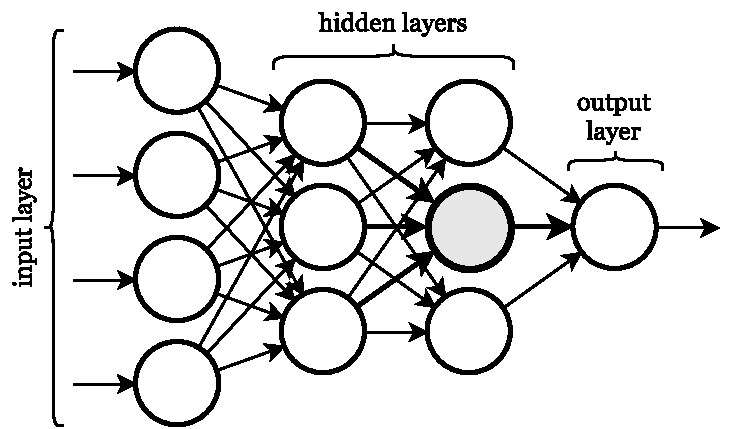
\includegraphics[width=.75\linewidth]{figures/mlp.pdf}
	\caption[Multilayer Perceptron]{Example of a MLP with two hidden layers. A single perceptron is highlighted in bold. (Based on \parencite{neural_nets_deep_learning})} \label{fig:mlp}
\end{figure}

The first and last layer of such a network are referred to as \textit{input layer} and \textit{output layer}. Furthermore, the number of nodes is determined by the given problem to solve. In case we want to train a network that identifies human faces in RGB-colored pictures with height and width of 100 pixels, it would require our input layer to have $ n_{in}=$ \num{30000} perceptrons, as well as a single output node. In contrary, all intermediate layers are known as \textit{hidden layers} and can have any number of elements and depth. When every node from one layer is connected to all nodes of its subsequent layer, it is called \textit{fully connected} (FC).

Afterwards, the input layer can be fed with a data example and apply equation \ref{eq:mlp} in each node to retrieve our binary result. This prediction step is called \textit{inference}. But in order to retrieve meaningful results, the network has to be trained first to have appropriate values for the weights and biases.

\subsection{Network Training}

The final goal of training such a network is to end up with a model that generalizes on any kind of data from the same type \parencite[p. 2]{pattern_and_ml}. Data that is used during this process is called \textit{training set}, the other portion of data that evaluates its generalization capabilities \textit{test set}. Additionally, a third split is preferably used during the training process of the networks to select the best performing approach. It is known as the \textit{validation set}. Since the ground truth outcome of each data example during the training phase is known, we can quantify the outcomes using a loss function\footnote{Often called cost function, objective function or error function as well.}, such as \textit{mean absolute error} (MAE)\footnote{Also known as $ \ell_1 $ when it does not average over all examples, but often used as a synonym. In this work, the averaged variants for all presented functions are always used. Additionally, we also average across the image pixels when any loss function is applied on images to achieve pixel-wise results that are independent regarding the image dimensions later on in context of frame prediction.}:

\begin{equation} \label{eq:mae}
  \mathcal{L}_{\textrm{mae}}(\textbf{w}, \textbf{b})=\frac{1}{n} \sum\limits_{\textbf{x}} | y(\textbf{x}) - t(\textbf{x}) | ,
\end{equation}

\textit{mean squared error} (MSE)\footnote{Also referred to as $ \ell_2 $ when no averaging across all examples is performed.}:

\begin{equation} \label{eq:mse}
  \mathcal{L}_{\textrm{mse}}(\textbf{w}, \textbf{b})=\frac{1}{n} \sum\limits_{\textbf{x}} ( y(\textbf{x}) - t(\textbf{x}) )^2 ,
\end{equation}

or \textit{binary cross-entropy} (BCE) \parencite{conv_lstm_nowcasting}:

\begin{equation} \label{eq:bce}
  \mathcal{L}_{\textrm{bce}}(\textbf{w}, \textbf{b})= -\frac{1}{n} \sum\limits_{\textbf{x}} t(\textbf{x}) \cdot \log{\big(y(\textbf{x})\big)} + \big(1-t(\textbf{x})\big) \cdot \log{\big(1-y(\textbf{x})\big)} ,
\end{equation}

where $ n $ is the number of examples and $ t(\textbf{x}) $ denotes a mapping from an input example $ \textbf{x} $ to its ground truth target. Many other functions exist and some more will be introduced in Section \ref{sec:perc-loss}, but the above listed formulas are the main objectives that are used in many other works. During training of the network, the set of weights $ \textbf{w} $ and biases $ \textbf{b} $ have to be found that minimizes the error:

\begin{equation} \label{eq:min-loss}
  \textrm{arg}\min_{\textbf{w}, \textbf{b}} \mathcal{L}(\textbf{w}, \textbf{b}) .
\end{equation}

Parameters beside $ \textbf{w} $ and $ \textbf{b} $ that are not learned during this process are called \textit{hyperparameters}. Examples of such non-trainable parameters are the number of layers or the size of each single hidden layer. More hyperparameters will arise throughout this chapter.


\subsubsection{Neurons and Activations}

At this point, the fundamental problem of perceptrons is faced. In order find the best set of parameters, small changes in the model's weights $ \textbf{w} $ and biases $ \textbf{b} $ have to be performed to justify the output into the right direction of the desired outcome. But since the perceptron's output is discrete, a small change can cause a sudden flip in the overall output of the model. To overcome this issue, these perceptrons are replaced with \textit{neurons}. The exemplary structure of a neuron is illustrated in Figure \ref{fig:neuron}. They are given by:

\begin{equation}
\begin{aligned}
z &= \sum\limits_{i=1}^n \, w_{i} \, x_{i} + b \\
y &= \phi(z) ,
\end{aligned}
\end{equation}

which allow $ x_{i}, y \in \mathbb{R} $ by wrapping its term with a non-linear \textit{activation function} $ \phi(z) $. Frequently used examples are the sigmoid function $ \sigma(z) $, hyperbolic tangent $ tanh(z) $ and the rectified linear unit (ReLU) $ max(0, z) $, illustrated in Figure \ref{fig:activations}.

\begin{figure}[htpb]
	\centering
	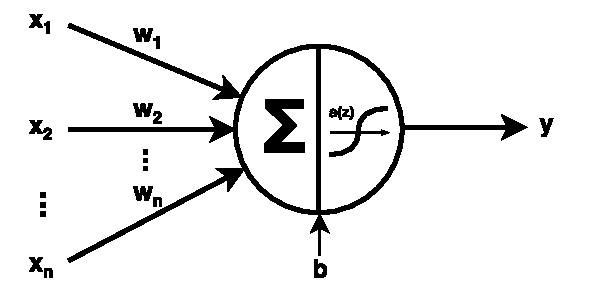
\includegraphics[width=.45\linewidth]{figures/neuron.pdf}
	\caption[Schematic Neuron]{Schematic structure of a neuron with its $ n $ inputs $x_{i}$, weights $w_{i}$, bias $ b $ and activation function $\phi(z)$.} \label{fig:neuron}
\end{figure}

Note that the sigmoid function's shape is a smoothed out variant of the \textit{step function} \parencite{neural_nets_deep_learning}, which can be used to make a neuron act like a classical perceptron. Additionally, the rectifier differs to both other activation functions in that it is one-sided and partly linear. Even that its shape looks much simpler, it became the most favorable activation function for intermediate layers in deep neural networks. The reasons are that it allows faster computation, sparse activation\footnote{{A sparse activation means that only half of the neurons have an initial non-zero output, when a uniform initialization is used.}}, reduces the likelihood of vanishing gradient (see Section \ref{sec:rnn-drawbacks}) and is more biologically plausible \parencite{relu}.

\begin{figure}[htpb]
  \centering
  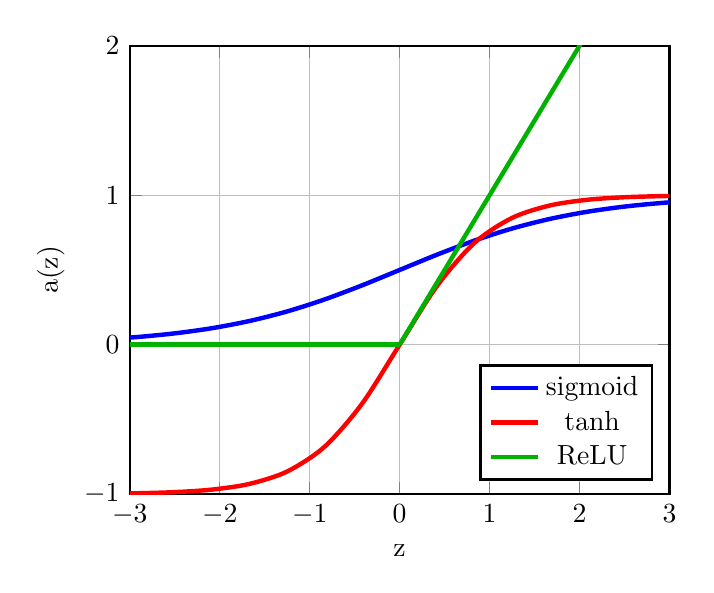
\begin{tikzpicture}
    \begin{axis}[
        ymin=-1,
        ymax=2,
        xmin=-3,
        xmax=3,
        legend style={legend pos=south east},
        grid,
        thick,
        ylabel=a(z),
        xlabel=z
      ]
      \addplot [mark=none,draw=blue,smooth,ultra  thick] {1/(1+exp(-1*(\x))};
      \addlegendentry{sigmoid};
      \addplot [mark=none,draw=red,smooth,ultra thick] {tanh(\x)};
      \addlegendentry{tanh};
      \addplot[mark=none,draw=black!30!green,ultra thick,smooth,domain=0:3] {x};
	  \addplot[mark=none,draw=black!30!green,ultra thick,smooth,domain=-3:0] {0};
      \addlegendentry{ReLU};
    \end{axis}
  \end{tikzpicture}
  \caption[Activation functions]{Visualization of the most commonly used activation functions in neural networks.}\label{fig:activations}
\end{figure}

\subsubsection{Initialization}

Before starting the training process, an initial value is assigned to each variable $ \textbf{w} $ and $ \textbf{b} $. This is done by pure randomness, using for example a uniform or Gaussian distribution. But if we start with weights that are too small, the signal could decrease so much that it is too small to be useful. On the other side, when we initialize our parameters with high values, the signal can end up to explode while propagating through the network \parencite{understand_xavier}. In consequence, a good initialization can have a radical effect on how fast the network will learn useful patterns.

For this purpose, some best practices have been developed. One famous example used in our final model is \textit{Xavier initialization}\footnote{Also known as Glorot initialization.} (see eq. \ref{eq:xavier}). Its formulation is based on the number of input and output neurons and uses sampling from a uniform distribution with zero mean and all biases set to zero \parencite{xavier-init}:

\begin{equation} \label{eq:xavier}
  \textbf{w} \sim \textrm{U} \bigg[-\sqrt{\frac{6}{n_{in} + n_{out}}}, \sqrt{\frac{6}{n_{in} + n_{out}}}\bigg] ,
\end{equation}

where $ \textbf{w} $ is the weight matrix at any network layer, $ n_{in} $ the number of incoming connections and $ n_{out} $ the number of outgoing connections to the next layer. This initialization is designed to keep the gradients in all layers within approximately the same scale.

As an alternative to random initialization and performing a training of the entire network from scratch, it is also possible to reuse parts or even all trained parameters from a different model. A famous example that is often used to pre-initialize a network for image processing tasks is \textit{AlexNet} \parencite{imagenet}. It is pre-trained for several weeks across multiple graphic cards on the large \textit{ImageNet}\footnote{ImageNet dataset: \url{http://image-net.org/}} dataset that contains 1.2 million images.

\subsubsection{Backpropagation Learning Algorithm}

To actually train the network by minimizing its error (see eq. \ref{eq:min-loss}), a learning algorithm called \textit{backpropagation} is applied. This algorithm is based on \textit{gradient descent}, which iteratively tries to find the minima of a function by doing small steps towards the negative gradient. Applying this to the given loss function results in the \textit{update rule} for any trainable weight and bias parameter:

\begin{equation} \label{eq:gradient_descent}
\begin{aligned}
w_{i}^{(\tau + 1)} &= w_{i}^{(\tau)} - \eta \cdot \frac{\partial \mathcal{L}}{\partial w_{i}^{(\tau)}} \\
b_{j}^{(\tau + 1)} &= b_{j}^{(\tau)} - \eta \cdot \frac{\partial \mathcal{L}}{\partial b_{j}^{(\tau)}} ,
\end{aligned}
\end{equation}

where $ \eta > 0 $ is the \textit{learning rate} that determines the step size that is done along the slope in each iteration \parencite{pattern_and_ml}. In other words, we proceed backwards through our network in every training iteration and slightly adjust every parameter depending on how much it has contributed to the error. Doing a single step by computing the gradients for the whole training set would require too much time and memory resources. Hence, the gradients are estimated over the whole population by using a smaller sample. This technique is called \textit{stochastic gradient descent} (SGD), whereas the size of the sample is known as \textit{batch size}.

Although this algorithm is really powerful, it comes with some disadvantages that have to be kept in mind. First, the result can converge to any local minimum. In consequence, finding a global minimum is not guaranteed. Secondly, depending on the choice of the learning rate $ \eta $, the algorithm might converge very slowly or even not at all \parencite{ann}.

Beside SGD, many other advanced gradient descent-based optimization algorithms exist. Detailed explanations  and visualizations can be found in \parencite{optimization}. The optimizer that is used in this thesis is called \textit{adaptive moments estimation} (Adam). This algorithm is based on adaptive estimates of lower-order moments and performs a form of step size annealing by using exponential moving averages of the parameters. Additionally, its hyperparameters $ \beta_1, \beta_2 \in [0, 1) $ have an intuitive interpretation and control the decay rates of the previous mentioned moving averages. Therefore, it usually requires less tuning of the learning rate or its other hyperparameters, and has shown to work very well in practice \parencite{adam}.


\subsubsection{Stopping Criteria}

The training process could basically run endless. Therefore, a rule should be defined when to stop it. There are many options when to cancel the training. Also, combinations of different \textit{stopping criteria} are possible. These can be for example:

\begin{itemize}
\item When the validation loss does not decrease (for a specified number of iterations).
\item When the change in loss falls below a defined threshold (for a specified number of iterations).
\item When a fixed number of steps or epochs\footnote{A single epoch is usually defined as the number of steps that is required to iterate over the whole training set.} elapses.
\item When a defined timeframe exceeds.
\end{itemize}


\subsection{Regularization}

As already stated, our goal is to find a representation that generalizes well. One common problem that has to be prevented when neural networks are trained is the effect of \textit{overfitting}. This means that even when the training loss decreases further and further, the validation and test error suddenly starts to get worse. One cause might be that the size of the training set is not large enough. But to come up with more data is often not possible. Another reason might be that our \textit{model complexity}\footnote{The complexity of a model is defined by the number of trainable parameters.} is too high. To get an idea about the reason for this, imagine we want to fit a function $g(x)$ using some noisy data points of a ground truth function $f(x)$. When our model exhibits to many parameters, it might come up with a function that perfectly fits to all given data points. Nevertheless, as demonstrated in Figure \ref{fig:overfitting}, this is a bad estimate of the underlying function $f(x)$.

\begin{figure}[htpb]
  \centering
  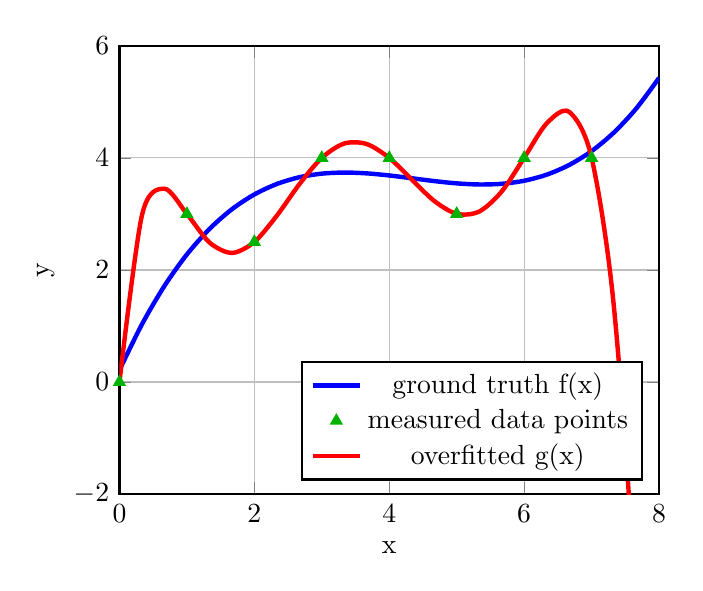
\begin{tikzpicture}
    \begin{axis}[
        ymin=-2,
        ymax=6,
        xmin=0,
        xmax=8,
        legend style={legend pos=south east},
        grid,
        thick,
        ylabel=y,
        xlabel=x,
        scatter/classes={%
		a={mark=triangle*,black!30!green}}
      ]
      \addplot [mark=none,draw=blue,smooth,ultra thick, domain=0:8] {
		 0.21212121212121271*x^0
   		+2.6607142857142843*x^1
  		-0.64502164502164450*x^2
   		+0.049242424242424192*x^3  
      };
      \addlegendentry{ground truth f(x)};
      \addplot[scatter,only marks,%
		scatter src=explicit symbolic]%
	table[meta=label] {
	x     y      label
	0     0      a 
	1     3      a
	2     2.5    a 
	3     4      a 
	4     4      a 
	5     3      a 
	6     4      a 
	7     4      a 
	};
	\addlegendentry{measured data points};
	\addplot [mark=none,draw=red,smooth,ultra thick, domain=0:8] {
		-0.0000000003717474*x^0
   		+14.921428855475133*x^1
  		-22.184722849828937*x^2
   		+13.906250509793455*x^3
  		-4.2638890895127091*x^4
   		+0.67083337448114122*x^5
  		-0.051388893117505295*x^6
   		+0.0014880954099440117*x^7
      };
      \addlegendentry{overfitted g(x)};
    \end{axis}
  \end{tikzpicture}
  \caption[Regularization and Overfitting]{Visualization of an overfitted function.}\label{fig:overfitting}
\end{figure}

On the other hand, a reduction of model complexity can also be a false conclusion because this limits the potential power of the network. Fortunately, research has originated different methods to master this issue. In the field of machine learning, these methods are referred to as \textit{regularization} techniques.

A well-known technique to delimitate overfitting is to penalize high parameter values which cause the oscillation effect that can be seen in Figure \ref{fig:overfitting}. Therefore, the loss function is extended with an additional regularization term. This method is called \textit{weight decay}:

\begin{equation} \label{eq:reg-loss}
  \mathcal{L}_{total}(\textbf{w}, \textbf{b})= \mathcal{L}(\textbf{w}, \textbf{b}) + \frac{\lambda}{n} \sum\limits_{\textbf{w}}\textbf{w}^2 ,
\end{equation}

where the coefficient $ \lambda $ controls the influence of the regularization. The term shown in equation \ref{eq:reg-loss} uses an $ \ell_{2} $ regularizer over all weights, which strongly penalizes a high magnitude of values. Together with the learning rate $ \eta $, both define two of the usually most significant hyperparameters in any neural network. Finding appropriate values is a major task when fine-tuning a model.

A second regularization approach is known as \textit{dropout}. Instead of modifying the cost function, it manipulates a specific layer of the model by randomly deactivating a neuron with a probability $p$ in every training step. As a result, the networks gets robust against distinct patterns that cause a high activation towards a certain output. Stated differently, the network is forced to not learn any shortcut that could damage generality. It is appropriate to add that no neuron is deactivated during inference. But to compensate the larger amount of active neurons within the layer, all weights of outgoing connections will be multiplied by factor $ p $ \parencite[p. 1931]{dropout}



\section{Convolutional Neural Networks}

In the previous section, neural networks have been discovered that exhibit a full connection of neuros from one layer to the next. While this allows to learn complex representations on the one hand, it comes with a couple of downsides on the other hand as well. For example, data such as images would require the layers of the network to become very large, especially in consideration of the input layer. Consequently, the number of connections between these layers would increase exponentially and thus the amount of trainable parameters as well. At the bottom line, this would end up in a network that is either time-consuming to train, or that is not even able to be stored in memory. In addition, it would not take any advantage of local image properties into account.

Therefore, a new network type found attention in recent years, which is known as \textit{convolutional neural network} (CNN). It is inspired by the animals' visual cortex, has already been used in the late 1990s to solve optical character recognition tasks (OCR) \parencite{lecun_conv} and received its main attention after beating proven methods in the \textit{ImageNet} competition by a large margin \parencite{imagenet}. The structure of a convolutional network, the detailed advantages and its mathematical formulation are described in the following sections.


\subsection{Structure}

A network is called CNN if it consists of at least one convolutional layer. In other words, ``\textit{convolutional networks are simply neural networks that use convolution in place of general matrix multiplication in at least one of their layers.}'' \parencite{deep_learning}. The definition of the convolution operation follows in Section \ref{sec:conv-op}. Simply put, imagine a small window that slides across the whole input space. In every iteration step, it attempts to extract features that are only dependent on a small neighboring region with the size of this window. Moreover, the location of features that it tries to detect is not fixed to any specific spot, as it treats every patch in the same way. In every convolutional layer, this process is repeated several times, resulting in multiple feature maps. Figure \ref{fig:cnn-structure} visualizes the described structure of a simplified convolutional neural network.

\begin{figure}[htpb]
	\centering
	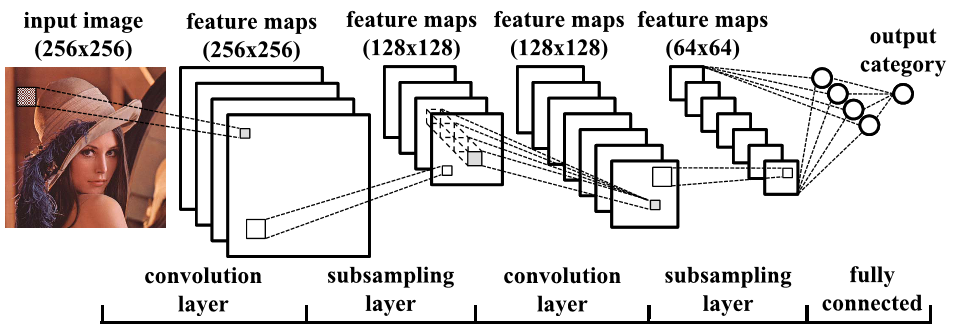
\includegraphics[width=1.0\linewidth]{figures/cnn_structure.png}
	\caption[Structure of a CNN]{Example of a simplified CNN structure with two convolutional layers for image classification. (Based on \parencite[p. 2284]{lecun_conv})} \label{fig:cnn-structure}
\end{figure}

The window mentioned before is called \textit{kernel} and holds the randomly initialized parameters that the network can learn. The kernel acts as a filter that is applied to each location in regular steps. In the two dimensional case, the kernel has a specified width and height, denoted as the \textit{kernel size}. Several kernels are used to extract multiple feature maps in each convolutional layer, but each output feature map is computed with its own kernel. This number of kernels is specified with its \textit{kernel depth}. Furthermore, the range the filter is moved in each dimension per step is called \textit{stride} \parencite{conv_guide}.

Each convolutional layer is usually followed by a non-linear activation function, preferably a rectifier. The reason is that the convolution is an affine transformation and is therefore linear. Stacking multiple linear operations could be mathematically reduced to a single one. Optionally, an additional \textit{pooling layer} can be applied that performs a subsampling onto the feature maps. Several pooling variants exist, while \textit{max pooling} is probably the most frequently used of them. It allows the representation to become roughly invariant to small rotations or translations of the input by only using the maximum value \parencite[p. 343]{deep_learning}.


\subsection{Convolution Operation} \label{sec:conv-op}

Generally speaking, a convolution in a mathematical operation on two functions $f(x)$ and $g(x)$. Its operator is typically denoted with an asterisk \parencite[p. 332]{deep_learning} and is defined as:

\begin{equation} \label{eq:conv-general}
  \big(f \ast g\big)(x) = \int f(\tau) \cdot g(x-\tau) \, d\tau .
\end{equation}

In terminology of convolutional networks, the function $f$ is termed as the \textit{input} and the filter $g$ is referred to as the \textit{kernel}. Moreover, the output of $ (f \ast g)(x) $ is called a \textit{feature map}.

As we are mainly dealing with discrete 2D images in this thesis, the formulation of equation \ref{eq:conv-general} can be discretized and reformulated as:

\begin{equation} \label{eq:conv-2d}
  \big(\textbf{I} \ast \textbf{K}\big)(x,y) = \sum\limits_{r=1}^{h} \sum\limits_{c=1}^{w} \textbf{I}_{c,r} \cdot \textbf{K}_{x-c,y-r} ,
\end{equation}

with an input $ \textbf{I} $ of size $w \times h$ and a two-dimensional kernel $ \textbf{K} $. Depending on the width and height of the kernel with a windows size of $ k \times k $ and the chosen stride $ s $, the shape of the convolved output changes. This is why the input is often enriched with zeros in order to have more control regarding the resulting output size. Surrounding the data with zeros is also known as \textit{zero-padding}. The use of no padding ($p=0$) is also called \textit{valid padding}, as depicted in Figure \ref{fig:conv_valid}. Also, when a padding of $p=\floor{k/2}$ is used that is half the kernel size, it is referred to as \textit{same padding}, shown in Figure \ref{fig:conv_same}. The reasons for its name is caused by the fact that the input and output size stay unchanged when a stride of $ s=1 $ is used.

\begin{figure}[htpb]
\centering
\begin{subfigure}{0.5\textwidth}
  \centering
  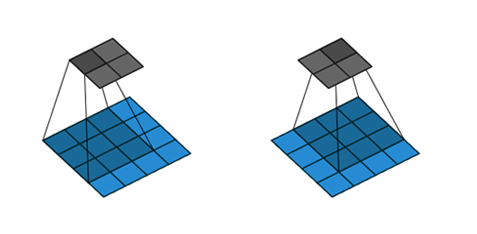
\includegraphics[width=.9\linewidth]{figures/conv_valid.png}
  \caption{$p=0$ (valid), $s=1$}
  \label{fig:conv_valid}
\end{subfigure}%
\begin{subfigure}{0.5\textwidth}
  \centering
  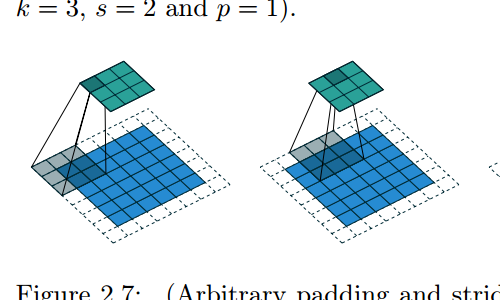
\includegraphics[width=0.9\linewidth]{figures/conv_same.png}
  \caption{$p=1$ (same), $s=2$}
  \label{fig:conv_same}
\end{subfigure}
\caption[Convolution Operation]{Visualizations of the convolutional operation with an $3 \times 3$ kernel but different settings for padding and stride. The white squares in (b) represent the padded zeros. (From \parencite{conv_guide})}
\label{fig:conv}
\end{figure}

It must be noted that the size of the kernel, padding and stride does not necessarily have to be equal in each dimension. But nevertheless, this is often the case in many practical applications.

\subsection{Transposed Convolution Operation}

The application of the previously presented convolution operation usually transforms the input into lower-dimensional feature maps. However, there are use cases where we would like to go the other way round, while keeping the connectivity pattern of a convolution. One application example is a convolutional autoencoder which is explained in further detail in Section \ref{sec:autoencoder}. This operation is referred to as \textit{transposed convolution}\footnote{Mistakenly, the transposed convolution is often called \textit{deconvolution}. But because it is not actually performing the reverse effect of a convolution, which is meant by the mathematical term of a deconvolution, it is strongly discouraged to name it so. An alternative name that is also often used is \textit{upconvolution}.}, which exchanges the forward and backward passes of a normal convolution. It is also called \textit{fractionally strided convolution}, because it can be emulated with a direct convolution using a zero-spaced input \parencite[p. 19]{conv_guide}. Such an implementation is less efficient, but it supports the intuition of how the resulting output shape looks like. Figure \ref{fig:conv_tp} shows an example of a transposed convolution.

\begin{figure}[htpb]
	\centering
	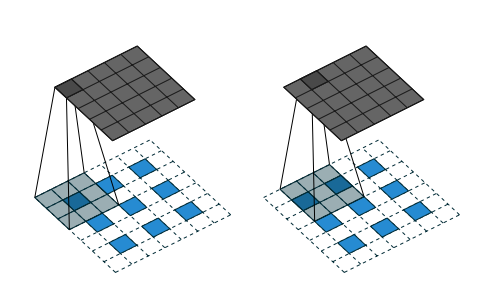
\includegraphics[scale=0.4]{figures/conv_tp.png}
	\caption[Transposed Convolution Operation]{Transposition of convolving an $6 \times 6$ input using a $3 \times 3$ kernel using $p=1$ and $s=2$. This is equivalent to performing a convolution using a zero-spaced $3 \times 3$ input with $p=1$ and $s=1$. (From \parencite{conv_guide})} \label{fig:conv_tp}
\end{figure}


\subsection{Advantages}

The three cenral design ideas are emphasized here to sum up the benefits of a convolutional network. It refers to \textit{sparse connections}, \textit{parameter sharing} and \textit{equivariance to translation} \parencite[p. 336ff.]{deep_learning}. The detailed advantages of these concepts are described in the following sections.

\subsubsection*{Sparse Connections}
The kernel size used in a convolution is smaller than the input. Consequently, less parameters have to be stored, as well as it can take advantage of local relationships present in the data. This also leads to a higher training efficiency and a radical reduction of memory requirements.

\subsubsection*{Parameter Sharing}
To handle all regions of the input data in the same manner, the parameters are \textit{reused} at every location as well. This is implemented by making use of only a single kernel which holds all learnable parameters.  Additionally, this \textit{weights sharing} decreases the number of parameters even further. To that end, Figure \ref{fig:conv_vs_fc} compares the connection pattern  and the sharing of model parameters of fully-connected layers against the convolutional case.

\begin{figure}[htpb]
\centering
\begin{subfigure}{0.5\textwidth}
  \centering
  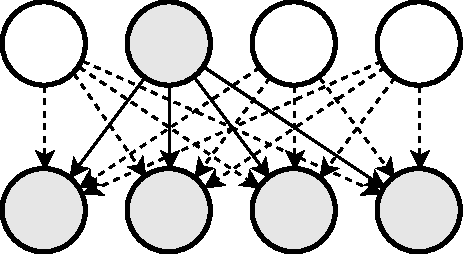
\includegraphics[width=.8\linewidth]{figures/fc2.pdf}
  \caption{}
  \label{fig:conv_vs_fc_fc}
\end{subfigure}%
\begin{subfigure}{0.5\textwidth}
  \centering
  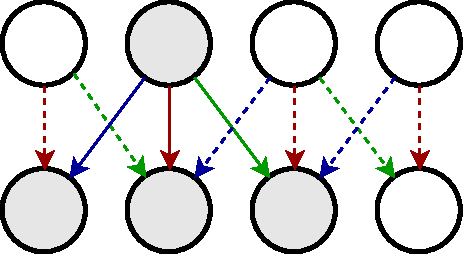
\includegraphics[width=0.8\linewidth]{figures/param_share.pdf}
  \caption{}
  \label{fig:conv_vs_fc_conv}
\end{subfigure}
\caption[Sparse Connections and Parameter Sharing in CNNs]{Comparison of the connection pattern and usage of parameters between (a) fully-connected layers and (b) convolutional layers. The use of the same color for interconnections denotes the sharing of parameters.}
\label{fig:conv_vs_fc}
\end{figure}

\subsubsection*{Equivariance to Translation}
The sharing of parameters leads to the third advantage. Because the kernel and its parameters are reused at every position, the model learns the same representations at every position \parencite[p. 339]{deep_learning}. For example, if an input image is translated by a fixed number of pixels, the network would handle it in the exact same way.

Unfortunately, convolutions are not tolerant to other transformations from the ground up. But to counteract these, other techniques exist such as a subsequent pooling stage to enable a slight rotation invariance, as already introduced before.


\subsection{Fully-Convolutional Networks}

The complete use of convolutional layers implicates a fourth advantage over fully-connected layers. Since the kernel size in each layer is independent regarding its input, the overall network could be fed with data of different dimension. In contrary, this is not possible anymore as soon as a single FC-layer is used at inference because its fixed-sized weight matrix has to be applied to the entire input, not just to a local region. Nevertheless, this does not imply that no fully-connected layer can be used at all when training the network. Depending on the architecture, FC-layers can be used in those parts of the network that are only used during training, but not when a prediction is performed while inference. This advantage is taken into account for example when a \textit{deep convolutional generative adversarial network} (DCGAN)\footnote{Novel network training strategy for generative networks. A generator network $ G $ competes against a second discriminator network $ D $ in an alternating fashion. Further details in \parencite{gan}.} is trained, whose discriminator network is only used in training mode.

Regarding the problem of frame prediction that has to be solved within this thesis, it has to deal with a huge amount of data in every training iteration. Therefore, the advantages from this \textit{fully-convolutional network} (FCN) approach are taken into account and design the architecture in such a way that it is possible to train the neural network model on small image patches only. Afterwards, it is theoretically able to perform frame prediction on the whole image given a sequence of frames.


\section{Recurrent Neural Networks}

All previously presented network architectures suffer from one missing characteristic: their memory is kind of static and predictions are mostly based on the current inputs only. Consequently, they are hard to be applied on problems where data reveals some sequential or temporal properties. Two examples are handwriting recognition, were the understanding of previous words is required to deduce the current word's context. Also in our case, the knowledge of the past image frames is fundamental to be able to predict the future frames that naturally match to the given previous sequence. A framework that addresses this issue is a \textit{recurrent neural network} (RNN). In this section, we give an overview about their structure and formal description, as well as present a succession model that addresses its fundamental problems. It is to add that the whole section is mainly inspired by the great explanations in \parencite{understand_lstm}.


\subsection{Basics}

RNNs are a special class of neural networks that allows its models to form a directed cyclic graph. Thereby, they are able to hold a hidden state that represents the sequential dynamics of the past. Given an input sequence $ \textbf{X} = (\textbf{x}^{(1)}, \textbf{x}^{(2)},..., \textbf{x}^{(\tau)}) $, the $ \tau^{th} $ recurrent building block gets $\textbf{x}^{(\tau)}$ as its input of this sequence, as well as the hidden state $\textbf{h}^{(\tau-1)}$ of the previous one. These building blocks are typically referred to as a \textit{cell}. Because the first cell has no predecessor, its hidden state input $ \textbf{h}^{(0)} $ is usually manually fed with an zero-initialized state vector. Formally, an RNN can be described as follows:

\begin{equation} \label{eq:rnn}
\begin{aligned}
\textbf{h}^{(\tau)} &= \phi(\textbf{W}_{h} \textbf{h}^{(\tau-1)} + \textbf{W}_{x} \textbf{x}^{(\tau)} + \textbf{b}_1) \\
\textbf{y}^{(\tau)} &= \textbf{W}_{o} \textbf{h}^{(\tau)} + \textbf{b}_2
\end{aligned}
\end{equation}

where $ \textbf{W}_{h} \in \mathbb{R}^{d_h \times d_h} $ are the weights of the hidden-to-hidden transitions, $ \textbf{W}_{x} \in \mathbb{R}^{d_x \times d_h} $ the weights of the input-to-hidden connections, $ \textbf{W}_{o} \in \mathbb{R}^{d_h \times d_x} $ the weights of the hidden-to-output transitions and $ \textbf{b}_1, \textbf{h}^{(0)} \in \mathbb{R}^{d_h}$ as well as $\textbf{b}_2, \textbf{x}^{(\tau)}, \textbf{y}^{(\tau)} \in \mathbb{R}^{d_x} $ the biases, initial state, input and output respectively \parencite[p. 2]{rnn-batchnorm}, \parencite[p. 381]{deep_learning}. The activation function $ \phi(\textbf{z}) $ is usually chosen to be a hyperbolic tangent.

Like convolutional networks, RNNs take advantage of sharing parameters over different parts of the model \parencite[p. 374]{deep_learning}. But in this case, model parameters are shared over the temporal domain. This allows the network to generalize specific properties across the whole input sequence. Consequently, a model can extract patterns that can occur at any or even multiple positions within the sequence of data.

\subsubsection{Structure}

For a better understanding of how recurrent networks work, it is helpful to take a closer look on its graphical model that was formally described by equation \ref{eq:rnn}. As it can be seen in Figure \ref{fig:rnn-loop}, the hidden state transition can be compactly visualized using a loop. These loops represent the influence of the past values with respect to the current value. However, to have a representation that is analogous to the already shown model, it is possible to unroll the loop in order to convert it back to a valid DAG. The unrolled recurrent network is depicted in Figure \ref{fig:rnn-unrolled}.

\begin{figure}[htpb]
\centering
\begin{subfigure}{0.26\textwidth}
  \centering
  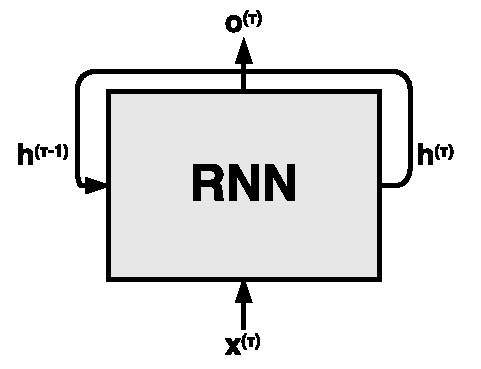
\includegraphics[scale=0.5]{figures/rnn_loop.pdf}
  \caption{}
  \label{fig:rnn-loop}
\end{subfigure}%
\begin{subfigure}{0.74\textwidth}
  \centering
  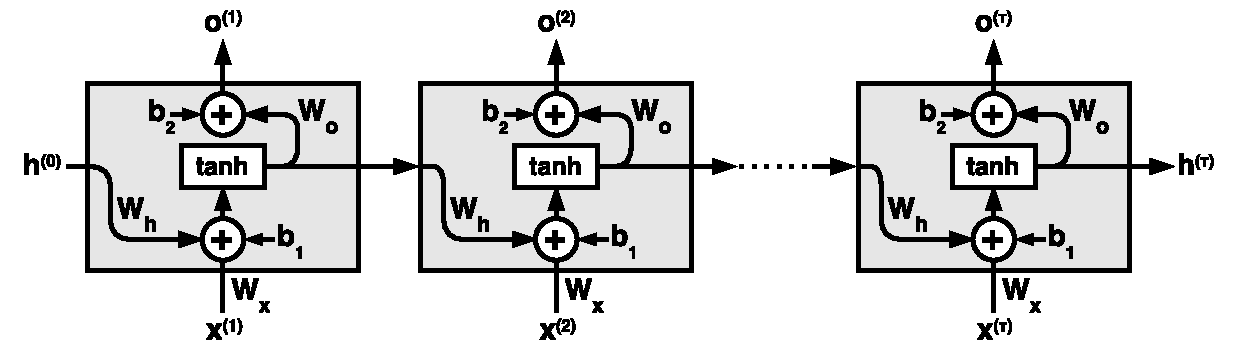
\includegraphics[scale=0.5]{figures/rnn_unrolled.pdf}
  \caption{}
  \label{fig:rnn-unrolled}
\end{subfigure}
\caption[Structure of Recurrent Cells]{Structure of recurrent network cells. The compact cyclic graph model in (a) can be unrolled to receive the model (b) that represents the network in form of an acyclic graph. (Based on \parencite{understand_lstm})}
\label{fig:rnn}
\end{figure}

In addition, the framework for recurrent models is very flexible as well. Depending on the implementation, it allows to process either a fixed or even a dynamic number of inputs. This property extends to the number of outputs as well. In contrary, convolutional or artificial neural networks require to define the input and output size at graph construction time. Further, they have to process all data in one chunk and do not allow to handle only single elements of the sequence one after the other. Some example input-output modes of recurrent networks are visualized in Figure \ref{fig:rnn-modes}.

\begin{figure}[htpb]
\centering
\begin{subfigure}{0.3\textwidth}
  \centering
  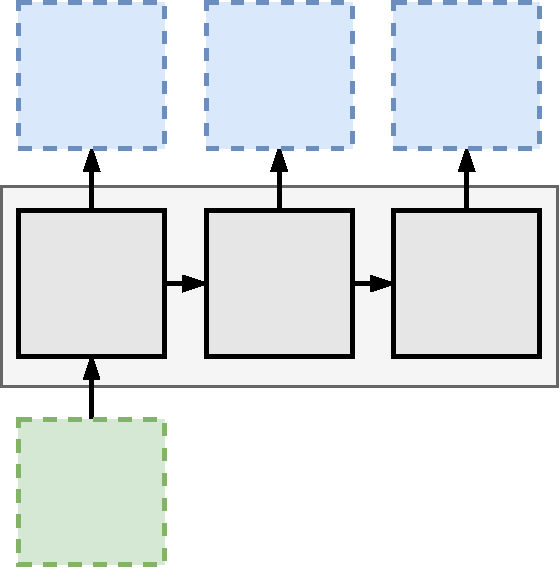
\includegraphics[width=.8\linewidth]{figures/one2many.pdf}
  \caption{}
  \label{fig:rnn-one2many}
\end{subfigure}%
\begin{subfigure}{0.3\textwidth}
  \centering
  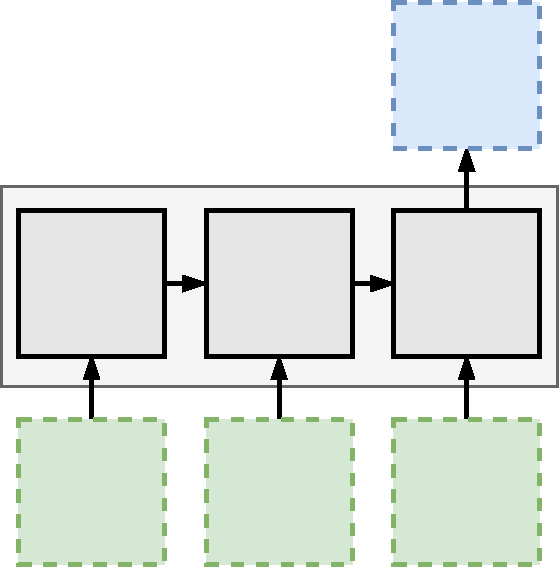
\includegraphics[width=.8\linewidth]{figures/many2one.pdf}
  \caption{}
  \label{fig:rnn-many2one}
\end{subfigure}
\begin{subfigure}{0.3\textwidth}
  \centering
  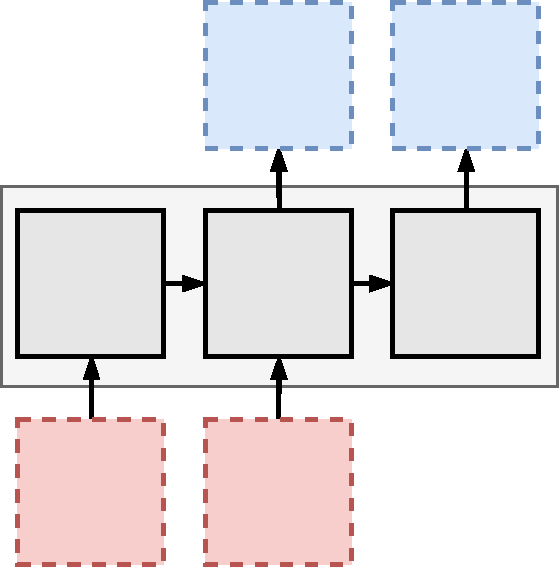
\includegraphics[width=.8\linewidth]{figures/many2many.pdf}
  \caption{}
  \label{fig:rnn-many2many}
\end{subfigure}
\caption[Examples of RNN Input-Output Modes]{Visualization of different recurrent network input-output modes: (a) one-to-many, (b) many-to-one, (c) many-to-many. Red squares denote the inputs, gray squares the recurrent cells and all outputs are colored in blue. Input and output squares can be understood as either further neural networks or the direct input and output. (Based on \parencite{rnn-effectiveness})}
\label{fig:rnn-modes}
\end{figure}

Besides the flexibility in the number of inputs and outputs, the recurrent components of the model is very adaptable as well. In common with the use of multiple neural network layers in order to achieve deeper and therefore more powerful models, several recurrent network layers can also be stacked on top of each other to enable a higher temporal depth. Various practical experiments, such as in \parencite{beyond_snippets_video_class}, \parencite{conv_lstm_nowcasting} or \parencite{unsup_learn_lstm}, have shown that \textit{multi-layer RNNs} are able to deliver better results compared to corresponding single-layer variants. Figure \ref{fig:rnn-multilayer} shows an example of a two-layer recurrent network. As a downside, the increase in the number of recurrent layers usually has a tremendous effect on the memory requirements and the network training time.


\begin{figure}[htpb]
\centering
\begin{subfigure}{0.3\textwidth}
  \centering
  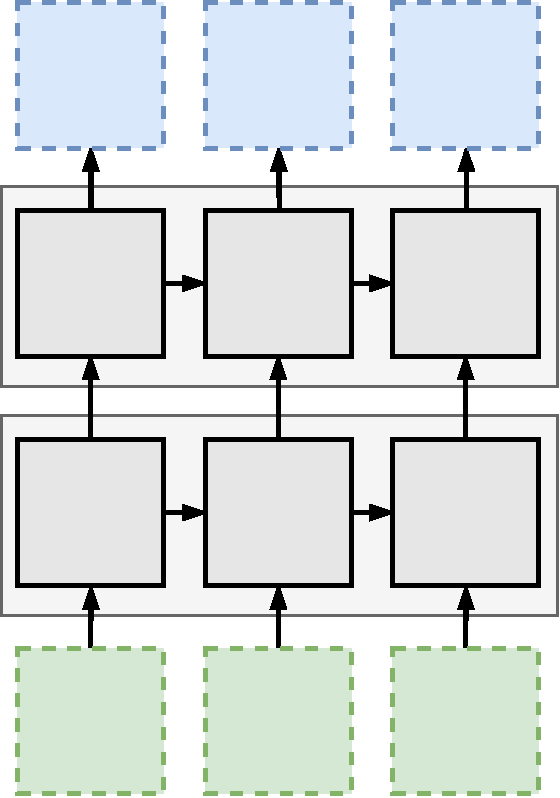
\includegraphics[width=.8\linewidth]{figures/rnn-multilayer.pdf}
  \caption{}
  \label{fig:rnn-multilayer}
\end{subfigure}%
\begin{subfigure}{0.3\textwidth}
  \centering
  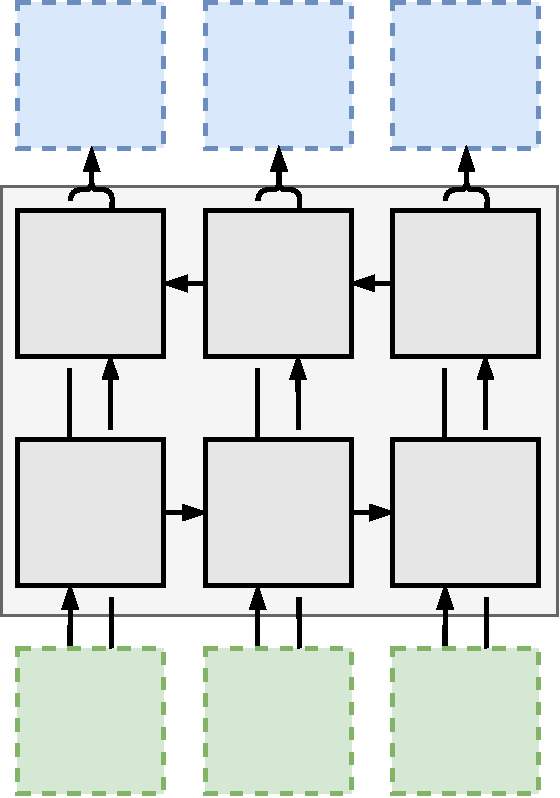
\includegraphics[width=.8\linewidth]{figures/rnn-bidirectional.pdf}
  \caption{}
  \label{fig:rnn-bidirectional}
\end{subfigure}
\caption[Deep Recurrent Network Architectures]{Examples of deeper recurrent network architectures. The figure in (a) shows a two-layer RNN, while (b) shows a single-layer BRNN. Both bidirectional outputs per cell of the latter model are combined and could be further processed by subsequent neural networks. (Based on \parencite{rnn-effectiveness})}
\label{fig:rnn-advanced}
\end{figure}

Additionally, the input sequence could be processed in both directions. This can be enabled by combining an RNN that starts at the beginning of the sequence with a second RNN starting from the very end backwards through time. In consequence, these so called \textit{bidirectional recurrent neural networks} (BRNN) are also able to have access to its future input information \parencite[p. 394ff.]{deep_learning}. It is to add that the recurrent weights are not shared in both directions. An example of such a bidirectional model is depicted in Figure \ref{fig:rnn-bidirectional}. The same idea could also be extended to a sequential processing of data in two dimensions, which is known as a \textit{grid RNN}.

\subsubsection{Backpropagation Through Time}

Analyzing the RNN structure might raise the question of how this effects the training procedure, because the gradient flows through recurrent cells multiple times while backpropagating the error. It is important to see that recurrent networks are still feed-forward networks with the extension to reuse the same weights expanded in time. Consequently, the error still has to be propagated backwards starting from the last time step $ \tau $ like in standard backpropagation. Depending on the length of the sequence and the computational resources, it can proceed until the very beginning, or truncate the view of interest by stopping at a given limit. Additionally, given the shared weights $ \textbf{w} $ of two timesteps $\tau $ and $ \tau+1 $, the weight constraint $ \textbf{w}^{(\tau)} = \textbf{w}^{(\tau+1)} $ must be met. Therefore, $ \nabla \textbf{w}^{(\tau)} = \nabla \textbf{w}^{(\tau+1)} $ has to be fulfilled as well. This can be realized by computing the gradients for both time steps independently, but use the average of the following sum:

\begin{equation} \label{eq:bptt}
	\frac{\partial \mathcal{L}}{\partial \textbf{w}^{(\tau)}} + \frac{\partial \mathcal{L}}{\partial \textbf{w}^{(\tau+1)}}
\end{equation}

when the final model parameter update is performed using the update rule \parencite{rnn-bptt}. This principle can be extended to the total sequence length that is considered by the recurrent network and is referred to as \textit{backpropagation through time} (BPTT).

\subsubsection{Drawbacks} \label{sec:rnn-drawbacks}

Keeping the previously explained weight constraints in mind, the recurrent network has to perform a lot of correlated updates of the same model parameters at once. This is actually bad for stochastic gradient descent, as it prefers uncorrelated parameters for the stability of the training. Especially when a sequence gets quite long, this can yield mathematical instability due to many multiplications using the same shared weights. On the one side, the gradients can grow exponentially and become infinite \parencite{lstm}. On the other side, the network could not learn anything because the gradients vanish. This issue is known as the \textit{vanishing and exploding gradient problem}. The lack of learning long-term dependencies in recurrent networks has been identified in \parencite{hochreiter} and \parencite{rnn-vanish}. Fortunately, other RNN variants exist that can deal with long-term dependencies. The currently most prominent version is introduced in the following section.


\subsection{Long Short-Term Memory}

Initially introduced by Hochreiter and Schmidhuber, the \textit{long short-term memory} (LSTM) became kind of the default recurrent network implementation as it is capable to deal with long range dependencies. Over the years, it has been revised by a couple of follow-up studies \parencite{lstm_peep} \parencite{lstm_v2} and is used in many practical applications today.

The central advancement of LSTMs over traditional recurrent networks is the so called \textit{memory cell state} $\textbf{C}^{(\tau)}$. While a simple RNN cell overrides its state at each time step, the LSTM's memory cell update exhibits only minor linear interaction, so that information could flow through very easily. Moreover, this simplifies the gradient flow backwards through time \parencite{rnn-batchnorm}. It follows that an LSTM cell inverts the core issue it tries to solve. Instead of learning to remember things, it is actually trained to learn what can be forgotten. In this way, keeping information over a longer period of time became its default setting.

To regulate the update of the internal memory state, the LSTM introduces the use of an attentive gating mechanism. At each time step, it is controlled by three trainable gates in order to accumulate or remove content from its state. Firstly, the \textit{input gate} determines the flow of information from the current input $ \textbf{x}^{(\tau)} $. Secondly, the \textit{forgot gate} regulates to which extend the information from the past cell state $\textbf{C}^{(\tau-1)}$ is kept. And lastly, the LSTM output state $\textbf{h}^{(\tau)}$ is specified by the filtered cell state using the \textit{output gate}. This mechanism allows constant error flow and enables to build a long-term understanding even when applied to long sequences. All this can be formalized as:

\begin{equation} \label{eq:lstm}
\begin{aligned}
\Spvek{\tilde{\textbf{f}}^{(\tau)}; \tilde{\textbf{i}}^{(\tau)}; \tilde{\textbf{o}}^{(\tau)}; \tilde{\textbf{c}}^{(\tau)}} &= \textbf{W}_{h} \, \textbf{h}^{(\tau-1)} + \textbf{W}_{x} \, \textbf{x}^{(\tau)} + \textbf{b} \\
\hat{\textbf{c}}^{(\tau)} &= tanh(\tilde{\textbf{c}}^{(\tau)}) \\
\textbf{C}^{(\tau)} &= \sigma(\tilde{\textbf{f}}^{(\tau)}) \odot \textbf{C}^{(\tau-1)} + \sigma(\tilde{\textbf{i}}^{(\tau)}) \odot \hat{\textbf{c}}^{(\tau)} \\
\textbf{h}^{(\tau)} &= \sigma(\tilde{\textbf{o}}^{(\tau)}) \odot tanh(\textbf{C}^{(\tau)})
\end{aligned} ,
\end{equation}

where $ \textbf{W}_h \in \mathbb{R}^{d_h \times 4d_h} $ are the shared weights for the hidden to hidden transitions at time step $ \tau $, $ \textbf{W}_x \in \mathbb{R}^{d_x \times 4d_h} $ the shared weights for the input to hidden connections, $ \textbf{b} \in \mathbb{R}^{4d_h} $ the biases, and $ \textbf{C}^{(0)}, \textbf{h}^{(0)} \in \mathbb{R}^{4d_h} $ the initial states of the memory cell and the hidden state, respectively \parencite{rnn-batchnorm}. The last dimension of the weight matrices and biases are multiples of four, because the matrices are concatenations of weights for all three gates plus the new candidate cell state $ \hat{\textbf{c}}^{(\tau)} $ for computational efficiency. The input, forget and output gates are labeled as $ \textbf{i}, \textbf{f} $ and $ \textbf{o} $. Furthermore, the operator $ \odot $ denotes the Hadamard product\footnote{The Hadamard product defines the entry-wise product of two matrices with the same dimension.} and a tilde indicates the term before the corresponding activation is applied, so that for example $ \textbf{f}^{(\tau)} = \sigma(\tilde{\textbf{f}}^{(\tau)}) $.


\subsubsection{Structure}

As depicted in Figure \ref{fig:lstm}, the internal structure of an LSTM cell looks way more complex compared to the simple RNN of Figure \ref{fig:rnn-unrolled}. Nevertheless, the role of each single building block has actually a quite simple interpretation.

\begin{figure}[htpb]
	\centering
	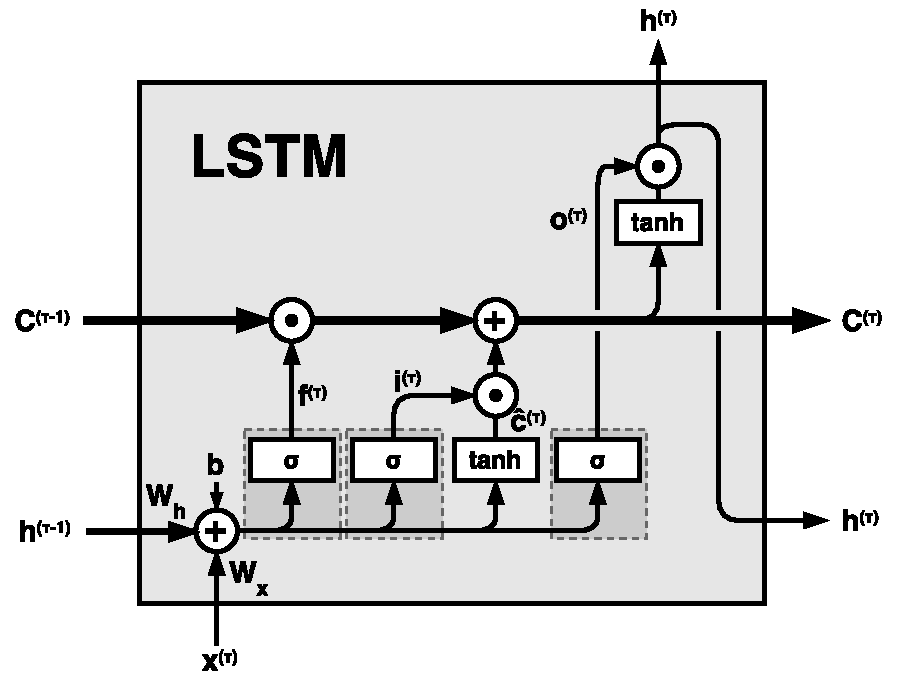
\includegraphics[width=.8\linewidth]{figures/lstm.pdf}
	\caption[Structure of a LSLTM Cell]{Structure of a LSTM cell. The flow of the cell state is highlighted in bold. Gated unites are emphasized with a dotted box. (Based on \parencite{understand_lstm})} \label{fig:lstm}
\end{figure}

As stated before, the fundamental enhancement of LSTMs is the cell state $\textbf{C}^{(\tau)}$, denoted as a bold line in the graphic. From its previous cell state to the next, there are just two interaction points where its content gets manipulated. First, using a pointwise multiplication with the output of the forget gate $\textbf{f}^{(\tau)}$, a specific part of the previous state can be partly or fully deleted. Afterwards, the new candidate cell state $ \hat{\textbf{c}}^{(\tau)} $ is added to it, which is only regulated by the input gate $ \textbf{i}^{(\tau)} $. The third gate $ \textbf{o}^{(\tau)} $ has no effect on the cell state itself and governs the hidden output only.
The interpretation of how each single gated unit works is the following: each gate itself is a fully-connected neural network layer, that receives the weighted sums of the input $\textbf{x}^{(\tau)}$ and the previous hidden state $\textbf{h}^{(\tau-1)}$ as its input. That is the reason why they are also often referred to as \textit{FC-LSTM}. Additionlly, as it can be seen in Figure \ref{fig:lstm}, every gate uses a sigmoid as its activation function that is followed by an Hadamard product. Consequently, the output of any gate is in range $ [0, 1] \in \mathbb{R}^{d_h \times 4d_h} $, where a value of one means let the whole information flow through, while zero intends to forget everything. 

\subsubsection{Variants}

The long short-term memory belongs to the family of \textit{gated RNNs} \parencite[p. 411]{deep_learning}. Since its invention, a couple of related implementations have been introduced. One example extends the LSTM by having so called \textit{peephole connections}, proposed in \parencite{lstm_peep}. These additional connections have the purpose that each gating unit has a direct access to the previous memory cell state $ \textbf{C}^{(\tau-1)} $. The motivation for this is to allow the units to learn when to open or close their gates based on the cell state \parencite{lstm-space}, in order to learn more precise timings.

Another example is the \textit{gated recurrent unit} (GRU) \parencite{gru}, which also regulates the flow of information comparable to an LSTM, but without having a separate memory cell. Additionally, its gates for input and output are merged to a single \textit{update gate}, which leads to a similar performance but with a lower memory footprint \parencite{gru-video}. The forgot gate in context of a GRU is typically called \textit{reset gate}.

A further, novel variant of LSTMs will be presented in Chapter \ref{chapter:implementation}, which is inspired by the strengths of convolutional neural networks. Aside from that, it will formalize the use of peephole connections as well.


\section{Encoder-Decoder Networks}

In order to learn useful representations, the generic, informative content has to be extract from the given data. But in many cases, we have to deal with a tradeoff between obtaining valuable properties and preserving as much information as possible regarding the inputs. Additionally, intense overfitting effects have to be handled when these representations are learned in a supervised fashion, because an acceptable amount of training data is often not on-hand for this purpose \parencite[p. 527]{deep_learning}. Therefore, this section focuses on concepts that are able to end up with good representations on the basis of unlabeled data in an \textit{unsupervised learning} process. 


\subsection{Autoencoders} \label{sec:autoencoder}

An \textit{autoencoder} is a commonly known neural network model that is able to reconstruct its own input. It consists of two components that are usually arranged in a mirrored style. First, an \textit{encoder} $ f(\textbf{x}) = \textbf{z} $ that maps any given input $ \textbf{x} \in \mathbb{R}^{d_x} $ to its internal representation $ \textbf{z} \in \mathbb{R}^{d_z} $. Second, a \textit{decoder} function $ g(\textbf{z}) = \textbf{x}^\prime $ that is able to map the representation back to its input. Due to the analogy to encoding and decoding, the learned representation is also often referred to as \textit{code}. In addition, the input and output layer of such networks have the same number of nodes. A simplified autoencoder model is visualized in Figure \ref{fig:autoencoder}. 

\begin{figure}[htpb]
	\centering
	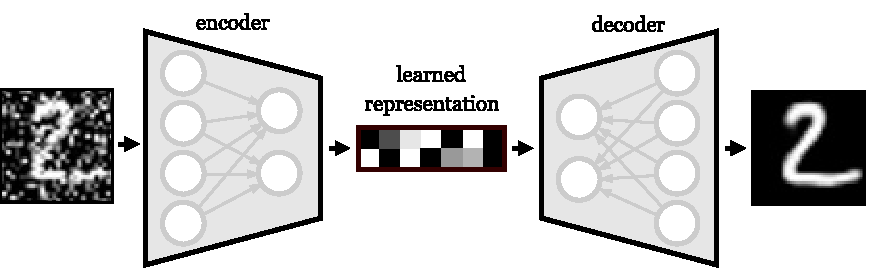
\includegraphics[width=.8\linewidth]{figures/encoder_decoder.pdf}
	\caption[Structure of an Autoencoder]{Simplified structure of a denoising autoencoder in an undercomplete setting to reconstruct images of handwritten numbers from the MNIST dataset.} \label{fig:autoencoder}
\end{figure}

The encoder and decoder components can be of any kind. In the simplest case, a neural network with only one single hidden layer could be used. However, it has been shown that deeper networks are able to yield better representations compared to shallow variants \parencite{autoenc_deeper}. Furthermore, the use of convolutional layers is usually preferred for image processing tasks, referred to as \textit{convolutional autoencoders}.

Reconstructing the input might sound trivial in first place. And honestly, the model itself that is able to learn the identity mapping $ g(f(\textbf{x})) = \textbf{x} $ and especially its output is not very interesting, since the network would just perform a copy operation. Instead, we are more interested in some special properties of the latent variable $ z $. These can be provoked by restricting the encoder, decoder or input with some additional constraints so that the model is not able to perform a perfect copy. Moreover, the dimensionality of the internal representation could be varied in order to force the model that it learns to prioritize which fraction of the input is worth to have in contemplation. Hence, it learns valuable properties regarding the data, which might even be useful to cope with other related tasks. Autoencoder models received increasing attention in recent years, especially in relation with \textit{generative models} \parencite[p. 502]{deep_learning}.

\subsubsection*{Undercomplete Autoencoders}

On the one side, in the typical \textit{undercomplete} case where the dimensionality of the representation is smaller than the input and output, so that $ d_z < d_x $, a model can be trained to reconstruct the original data \parencite[p. 503]{deep_learning}. As an application example, this can yield in an image compression algorithm, where the encoder compresses an input image to another representation of lower size. Afterwards, the decoder network can be used to recover the image data. As a result, depending on how much lower the size of the representation and the dissimilarity of the reconstruction compared to its original image is, the better is our learned representation. It then would have learned to preserve the image information in a more compact way.

\subsubsection*{Regularized Autoencoders}

On the other side, there are also use cases for \textit{overcomplete} models where the representation's dimensionality could exhibit an equal or even higher dimension than the input and output\footnote{It is to be added that the presented regularization strategies can also be used for undercomplete autoencoders.}, so that $ d_z \geq d_x $. But this requires to apply regularization techniques in order to learn useful features. The reason is that such a high model capacity can easily end up in overfitting \parencite[p. 504f.]{deep_learning}. One first possibility is to extend the loss function with an additional sparsity penalty, so that the \textit{sparse autoencoder} network tries to minimize:

\begin{equation} \label{eq:autoenc-sparse}
	\mathcal{L}(\textbf{x}, g(f(\textbf{x}))) + \lambda \cdot \Omega(\textbf{z}) ,
\end{equation}

where $ \lambda $ controls the tradeoff between sparsity and reconstruction and regularizer term $ \Omega(\textbf{z}) $ can be any valid loss function, such as $ \ell_2 $. This sparsity constraint reduces the autoencoder's degrees of freedom and therefore prevents overfitting. To put it another way, the model is virtually undercomplete by having a compactly distributed representation instead of a lower dimensionality. Alternatively, sparsity could also be achieved by only using the $ k $ most meaningful activations in a \textit{k-sparse autoencoder} by zeroing out weak hidden units manually \parencite{k-sparse-autoenc} or by using rectifier units in the last encoding layer \parencite{rect-autoenc}.

A second regularization strategy is to modify the reconstruction term of the loss function itself by adding random noise to the input. These networks are called \textit{denoising autoencoders} and have to learn how to correct back the added noise for the purpose of reconstructing the original noise-free image \parencite[p. 507]{deep_learning}. Therefore, the network has to learn a deeper understanding of the input data instead of simply copying its content. As a consequence, it has to minimize:

\begin{equation} \label{eq:autoenc-denoise}
	\mathcal{L}(\textbf{x}, g(f(\tilde{\textbf{x}}))) ,
\end{equation}

where $ \tilde{x} $ is the randomly corrupted version of the ground truth input $ x $.


\subsection{Recurrent Encoder-Decoder Models} \label{sec:rnn_enc_dec}

The general idea of the encoder-decoder framework can also be applied to recurrent networks. Thus, it can build a complex representation by incorporating a whole sequence of inputs. To our knowledge, the \textit{recurrent encoder-decoder} model has been firstly introduced independently from each other in \parencite{brnn_fist} and \parencite{brnn_second}. Further, it has been used in  \parencite{unsup_learn_lstm}\footnote{The authors call this recurrent framework the \textit{LSTM autoencoder model} within their publication. But due to the fact that it can be generalized to another recurrent cell implementations, as well as it could be applied in a non-autoencoder fashion, the more general name \textit{recurrent encoder-decoder} model is used here as well. This name is also used in several follow-up works.} for the first time in context of image processing. But since then, it has been applied in numerous subsequent works \parencite{rnn-enc-dec1}, \parencite{rnn-enc-dec2}. Figure \ref{fig:rnn-autoencoder} shows an example of such a model in context of a recurrent autoencoder.

\begin{figure}[htpb]
	\centering
	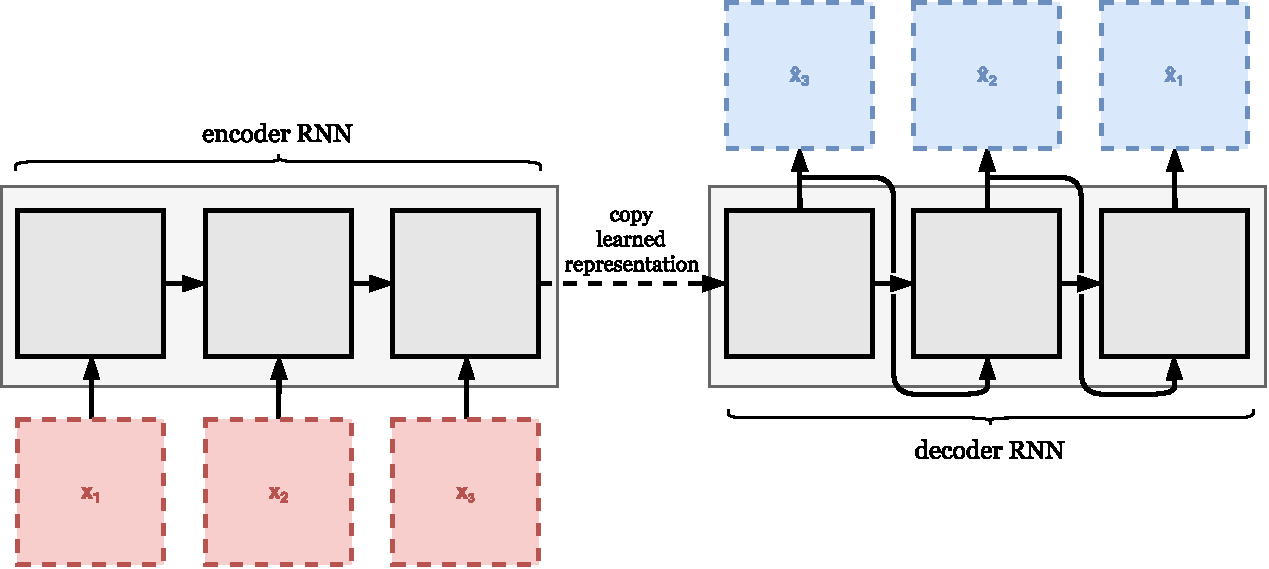
\includegraphics[width=.9\linewidth]{figures/rnn_autoencoder.pdf}
	\caption[Recurrent Autoencoder Model]{Basic structure of a conditional recurrent autoencoder. The inputs (red) are processed by the encoder RNN to learn the representation of the data in sequence. Then, the decoder RNN takes over to infer the reconstructions (blue) of the inputs in reverse order. (Based on \parencite{unsup_learn_lstm})} \label{fig:rnn-autoencoder}
\end{figure}

The encoder RNN builds the representation based on all inputs of the sequence and therefore takes advantage of its temporal or ordinal structure. Afterwards, the learned representation is used to initialize the hidden state $ \textbf{h}_{\textrm{dec}}^{(0)} $ of the decoder, in opposite to the otherwise customary zero initialization. The decoder RNN takes then over and outputs the prediction of the target sequence. Obviously, both the encoder and decoder recurrent networks could be extended to consist of multiple layers or bidirectional connections as well.

There are at least two possibilities of how the decoder can be designed. Firstly, an unconditional setting where each recurrent cell does \textit{not} receive the previous output as its input. Secondly, a conditional setting in which this additional connection from the cell's output to the input of the next element is present. Both have its reasons for and against. On the one side, it can be argued that conditioning on the previous output enables to learn more dynamics in the target sequence distribution. This conditioning might not be required in an autoencoder setting, where there is only exactly one ground truth target sequence. But when this architecture is applied to continue a series of frames in the future, it could be crucial to have access to the previous output. As an example, consider the prediction of a series of frames from a simple video game, where the player could walk either left or right in a specific situation. To properly predict the next outputs afterwards, it is fundamental to know which decision this particular recurrent cell has made. Otherwise, the RNN might end up in averaging over all possible outcomes. On the other side, it could also be argued that conditioning on the previous frame would end up in preventing the network to look deeper inside the encoder network \parencite{unsup_learn_lstm}.


\section{Batch Normalization}

Training a deep neural network model is said to be very hard. One reason for this is that every layer has not just to learn the overall representation directly from the beginning of the training, but also has to master the continuous change in distribution of its inputs, given all preceding layers. As an example, consider one layer in the middle of a deep network. At training time, its adjustments to the model parameters depend on its inputs, which is equivalent to the output of the previous layer. But the fact that the previous layer learns and modifies its weights and biases, it follows that the input to the following layer can change over time significantly. Especially at the very beginning of the training, due to the common use of random initialization. This ongoing change in the feature's distribution during training is known as the \textit{internal covariance shift} \parencite{rnn-batchnorm}.

One modern practice that tries to overcome this issue is called \textit{batch normalization} \parencite{batchnorm}. It performs a normalization on the inputs to a layer and transforms it to have a mean of zero and a standard deviation of one. Consequently, it compensates the covariate shift between two layers of the network. Its mathematical formulation is:

\begin{equation} \label{eq:bn}
\textrm{BN}(\textbf{x}; \gamma, \beta) = \beta + \gamma \frac{\textbf{x} - \mathbb{E}(\textbf{x})}{\sqrt{Var(\textbf{x}) + \epsilon}} ,
\end{equation}

where $ \textbf{x} \in \mathbb{R}^d $ is the output of the previous layer to be normalized, $\gamma \in \mathbb{R}^d $ and $\beta \in \mathbb{R}^d $ the learned shift and scale of the distribution, as well as $\epsilon \in \mathbb{R} $ that serves as a regularization parameter to avoid dividing by zero \parencite{rnn-batchnorm}.

When batch normalization is applied, two different modes during training and inference have to be considered. On the one hand at training time, batch normalization takes advantage of two simplifications, caused by the fact that full whitening of the inputs is very expensive. First, each feature dimension is normalized independently. Secondly, the statistics of $ \mathbb{E}(\textbf{x}) $ and $ Var(\textbf{x}) $ are estimated using the sample mean and sample variance based on each mini-batch of stochastic gradient training. On the other hand, the statistics have to be assessed using the entire training data during inference. One way to do so is to track the moving averaged mean and variance parameters of each batch-estimate while training the model, and finally use these averaged values when a prediction is performed. This is the way how batch normalization is used throughout this work.

The advantages of batch normalization are versatile:

\begin{itemize}
\item Compensation against internal covariate shift to achieve a stable distribution of activation values.
\item Separate normalization of individual feature dimensions, so that features are not decorrelated.
\item Speed-up training, because it allows to use higher learning rates.
\item Practice has shown that even a higher accuracy can be achieved compared to non-batch-normalized versions of a network model \parencite[p. 7]{batchnorm}.
\end{itemize}


\section{Image Similarity Assessment}

The practical use of deep learning in context of image generation tasks received a tremendous increase in recent years. Examples include denoising autoencoders (see Section \ref{sec:autoencoder}) for image reconstruction, semantic image completion \parencite{sem-img-inpainting}, the determination of optical flow \parencite{flownet}, \parencite{flow-static-img} or future  frame prediction of a given image sequence. The last mentioned field of application is in scope of this thesis. 

A neural networks main driver in respect to learning a good representation is the loss layer. Unfortunately, it found only little attention in most existing studies when applied in image processing tasks, at least until this year \parencite{loss-func-img-proc}. Therefore, this section provides an overview of the main challenges of image similarity assessment and introduces some approved methods, as well as novel approaches when training neural networks in context of pictures.


\subsection{Naive Approach}

The de facto standard loss function to compare a generated image with its ground truth target has been the \textit{pixel-wise squared error} (or $ \ell_{2} $) that was already mentioned in equation \ref{eq:mse}. It is easy to apply and usually provided by any neural network framework out-of-the-box. But as a downside, it suffers from some well-known limitations such as poor correlation with the human sense of perceptual quality \parencite{loss-func-img-proc}. The reason for this are twofold. First, $ \ell_{2} $ makes the assumption of a Gaussian noise model, which has its downsides when being applied to multimodal distributions. Second, it strongly penalizes outliers independently from local characteristics of the image, such as contrast or luminance. In contrary, the visual system of humans perceives noise in a different way.

\begin{figure}[htpb]
\centering
\begin{subfigure}{0.5\textwidth}
  \centering
  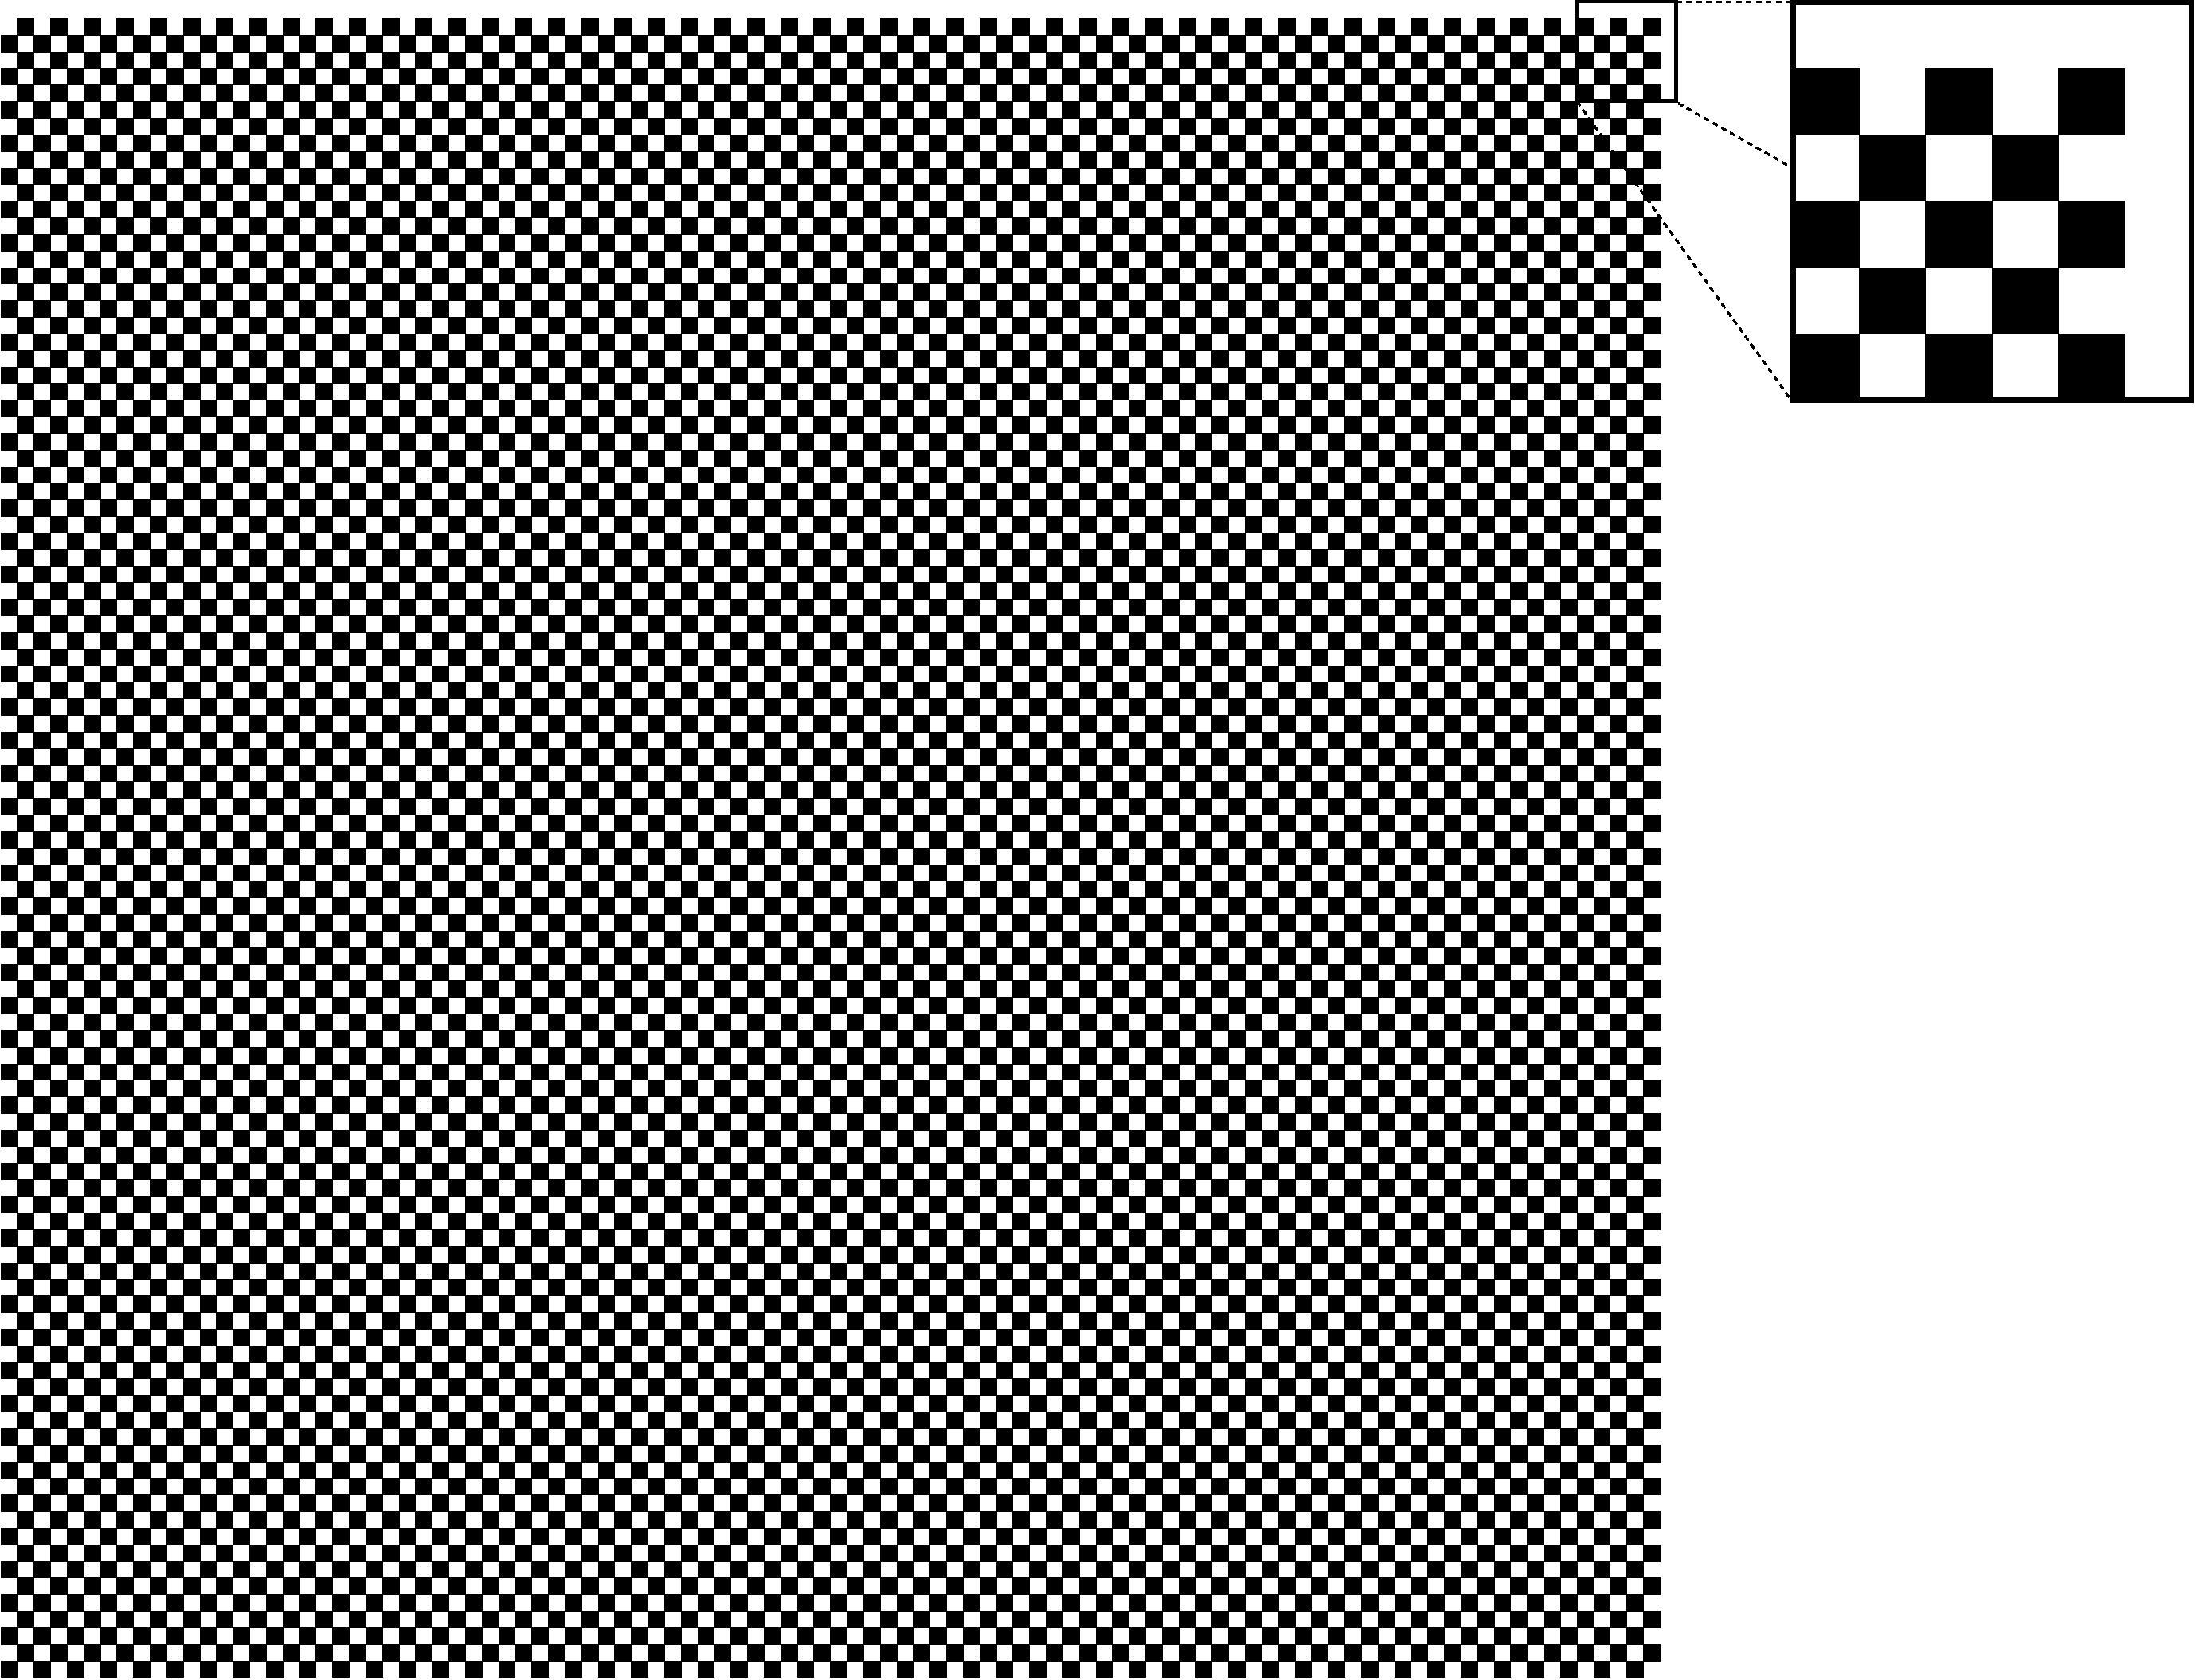
\includegraphics[width=.8\linewidth]{figures/chess1.pdf}
  \caption{}
  \label{fig:chess1}
\end{subfigure}%
\begin{subfigure}{0.5\textwidth}
  \centering
  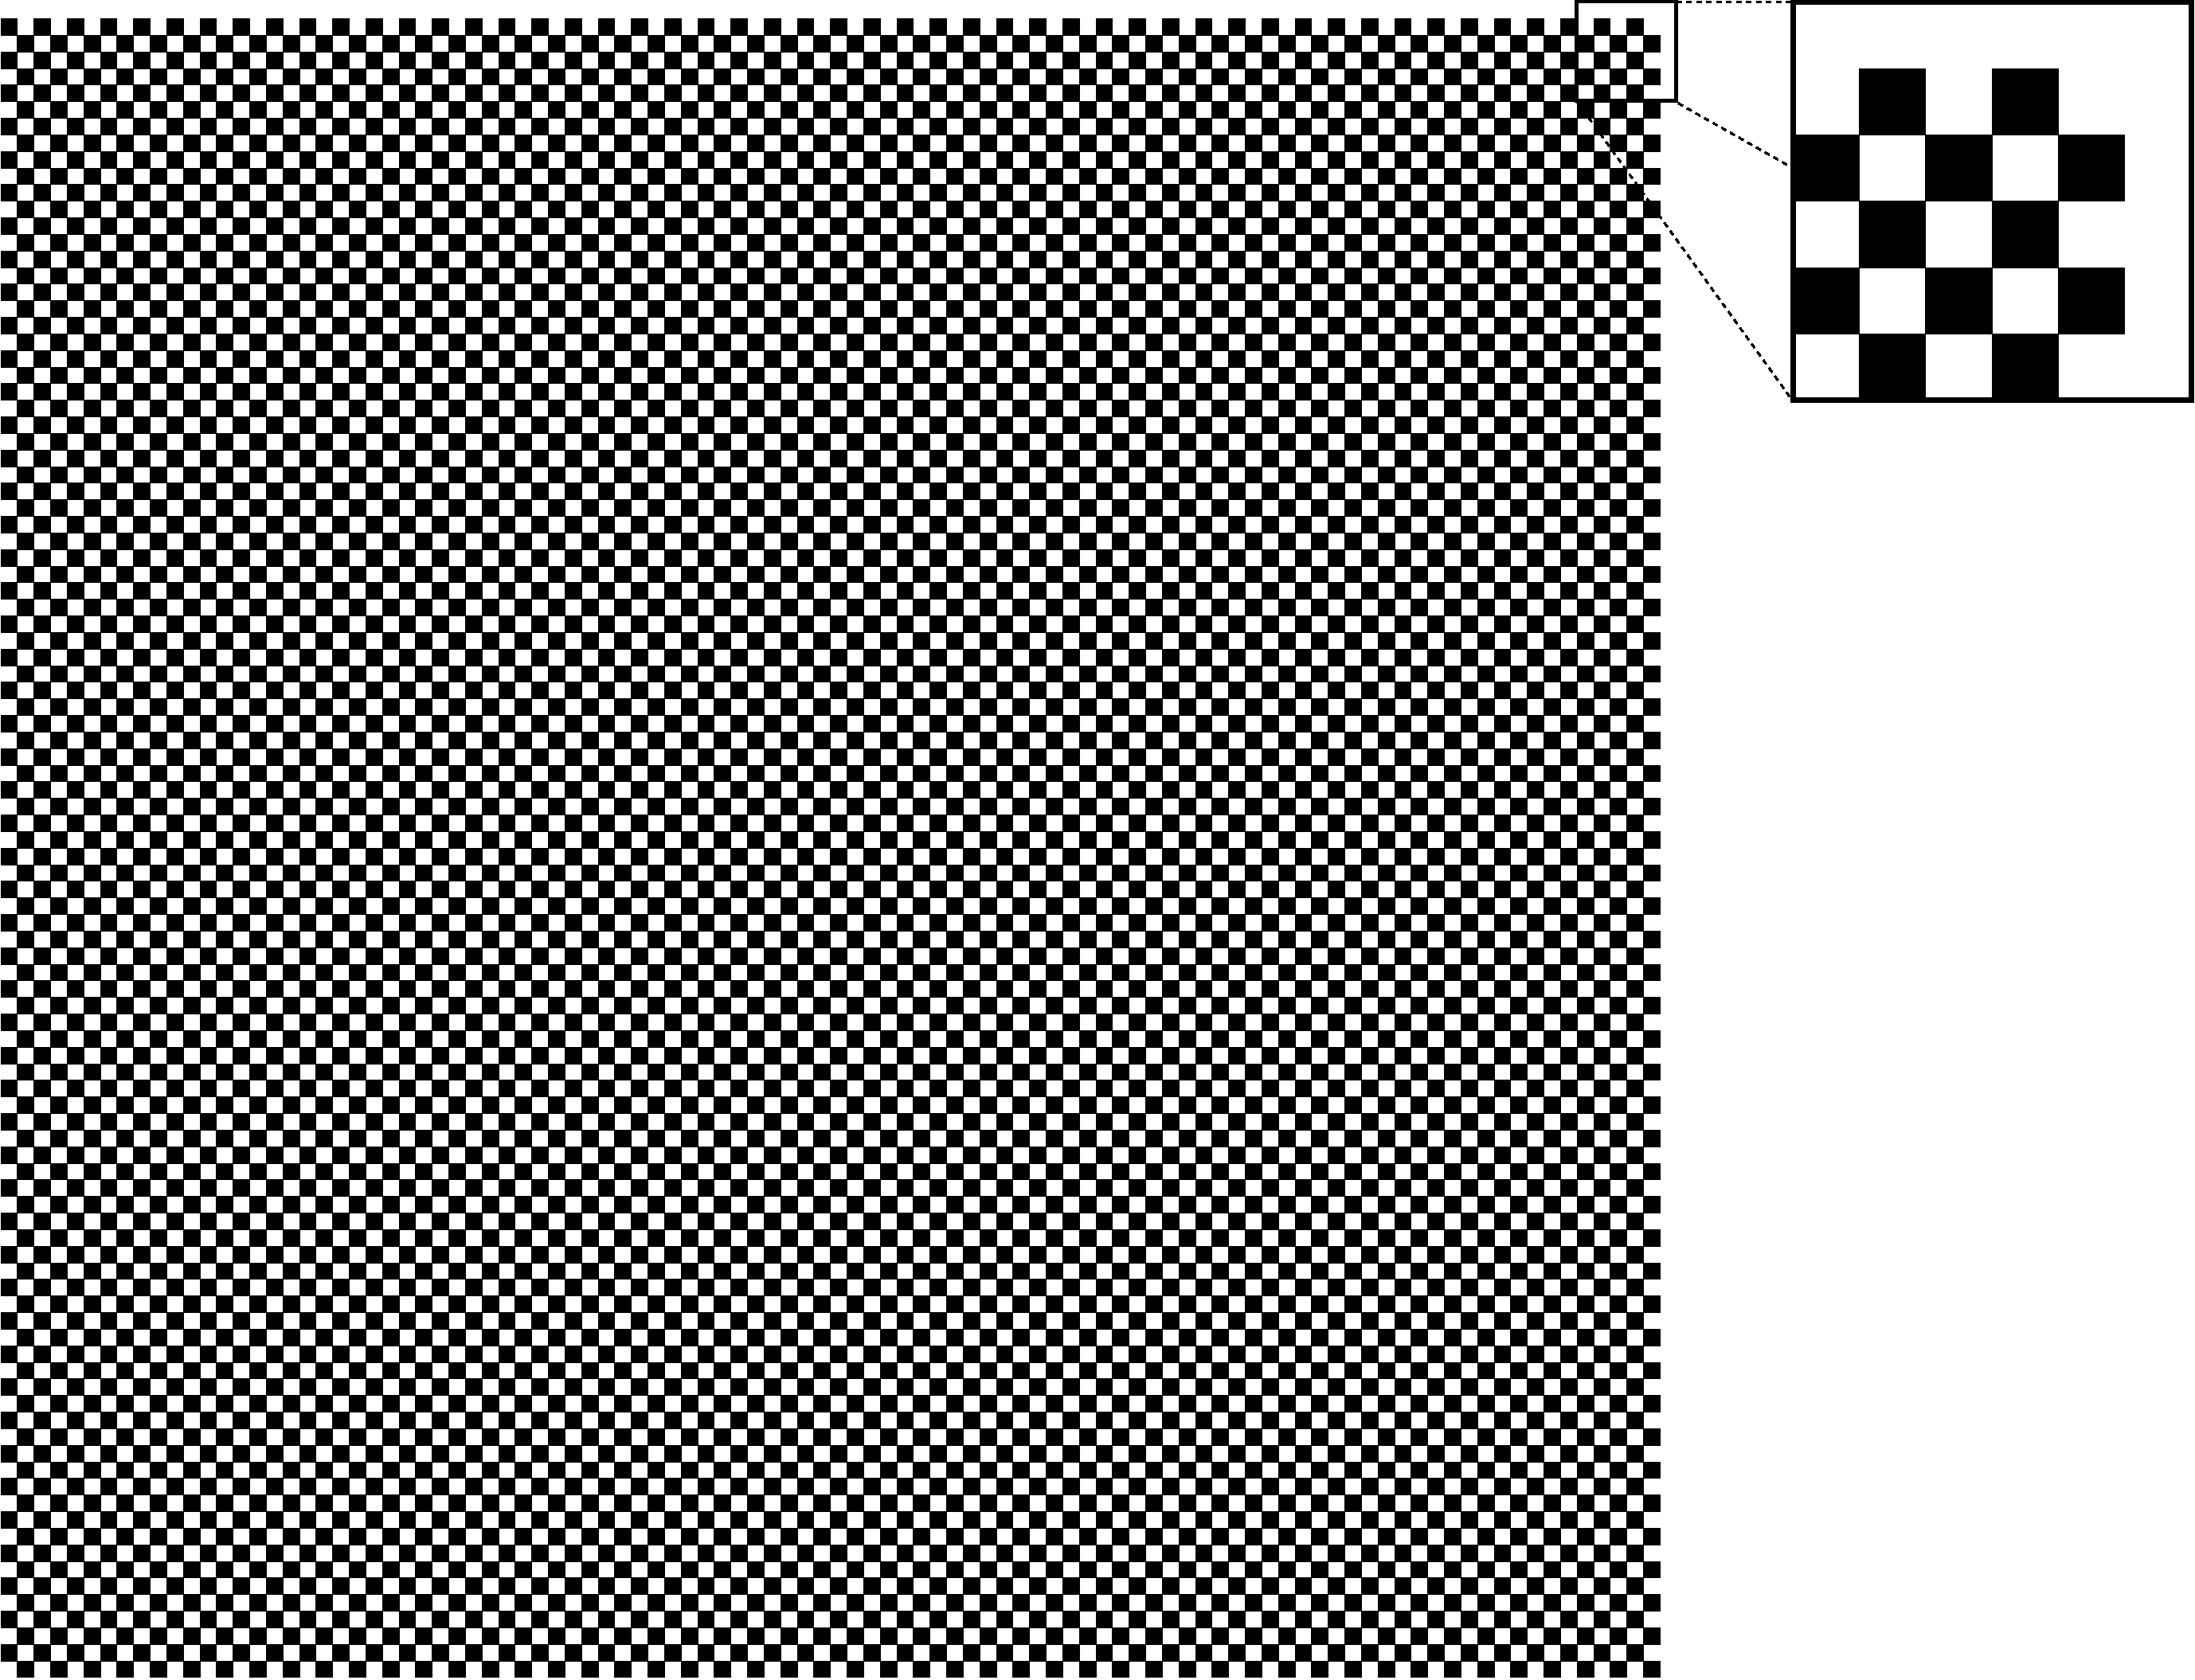
\includegraphics[width=.8\linewidth]{figures/chess2.pdf}
  \caption{}
  \label{fig:chess2}
\end{subfigure}
\caption[Example of $ \ell_{2} $ Weakness]{Example to demonstrate the weakness of $ \ell_{2} $ in context of perceptual image similarity.} \label{fig:chessfield}
\end{figure}

As an extreme but simple example, consider two images containing a chess field of black and white pixels as shown in Figure \ref{fig:chessfield}. From an aerial perspective, both images look completely identical, because it is perceived as a gray surface. Additionally, even when we look at it from a closer distance, we would still evaluate them as quite similar. This is for the very reason that both images provide the same colors, structure, sharpness or contrast. Unfortunately, assessing both images using the given squared error function results in the maximum possible difference. The reason for this is because it considers the squared differences of related pixels only. Even that this specific weakness is not solved by using the $ \ell_{1} $ loss, several studies have shown that the usage of the absolute error function slightly reduces the blur effect on edges in image generation processes of natural images \parencite{loss-func-img-proc} \parencite{deep_multiscale_video_pred}. Some example image reconstructions comparing the use of different loss functions are show in Figure \ref{fig:percept-vs-lp}.

\begin{figure}[htpb]
\centering
\begin{subfigure}{0.4\textwidth}
  \centering
  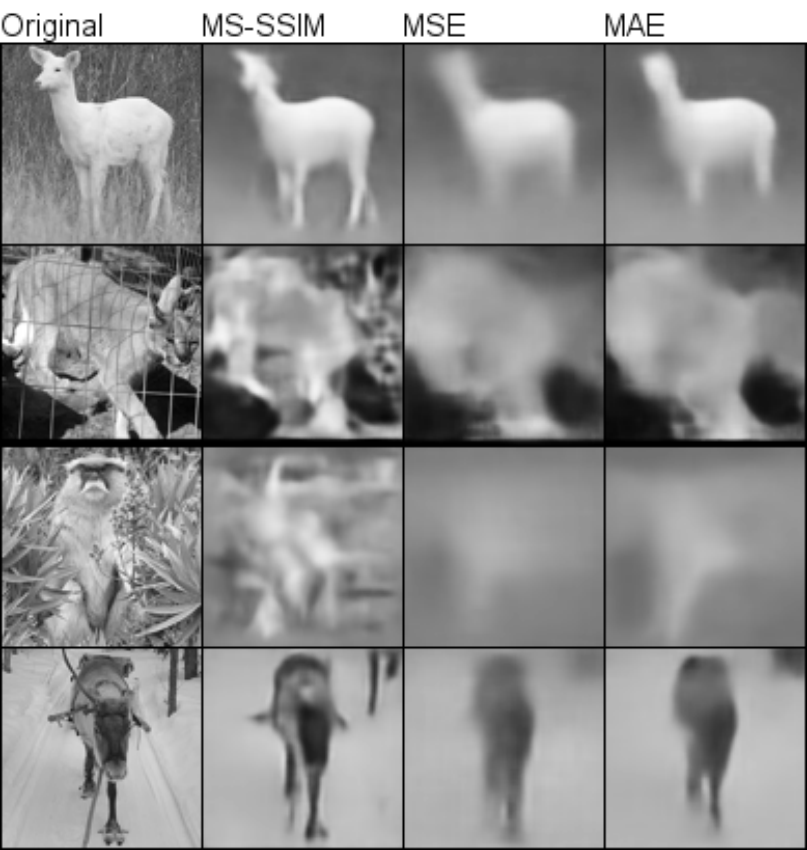
\includegraphics[width=.8\linewidth]{figures/img-loss-comp1.png}
  \caption{}
  \label{fig:percept-vs-lp1}
\end{subfigure}%
\begin{subfigure}{0.4\textwidth}
  \centering
  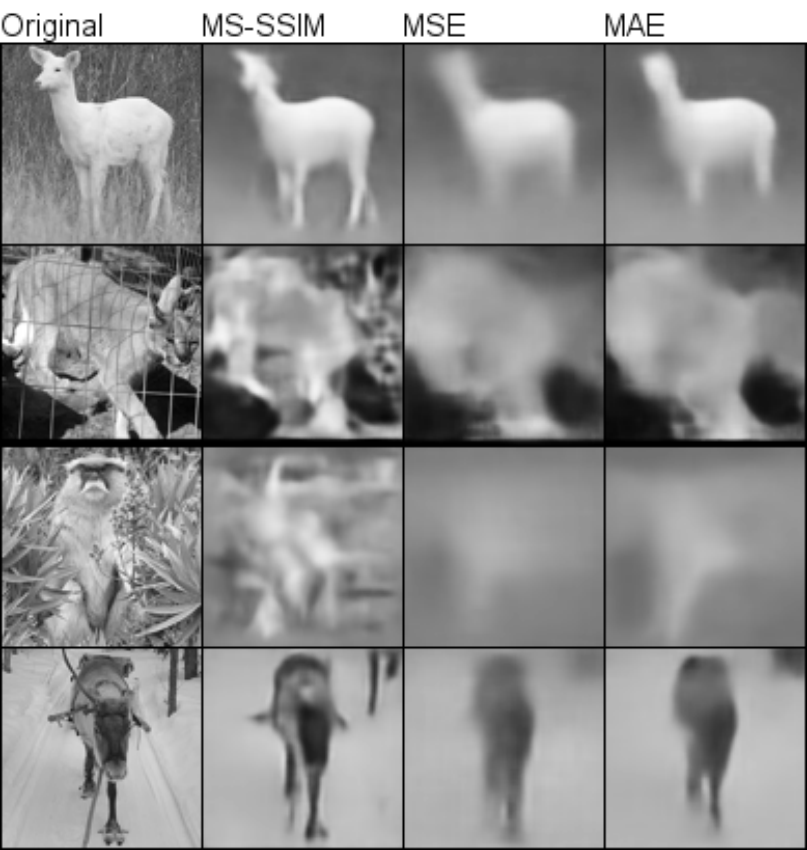
\includegraphics[width=.8\linewidth]{figures/img-loss-comp1.png}
  \caption{}
  \label{fig:percept-vs-lp2}
\end{subfigure}
\caption[Comparison of Reconstructions with Different Loss Functions]{Comparison of reconstructions with different loss functions using images from the STL-10 dataset: (a) where results using a perceptual motivated loss function were ranked first by human judgement, (b) where MAE or MSE were ranked best. (From \parencite{learning-perc-sim})}
\label{fig:percept-vs-lp}
\end{figure}


\subsection{Perceptual Quality Metrics}

The example in the previous section has shown that the consideration of the human visual perception is very important when assessing image similarity. With this in mind, a couple of metrics have been developed to evaluate image quality differences between two images. These metrics can be used either for a quantitative evaluation of generated results, or even as a loss function by doing some minor modifications to fulfill the required properties. Beside neural network training, these metrics have been originally invented to measure the quality of image compression codecs such as JPEG\footnote{JPEG: stands for \textit{Joint Photographic Experts Group} and is the name of the committee that created this compression standard for digital pictures.}.

In the following sections, $ \textbf{x} $ will denote the ground truth image and $ \textbf{y} $ its generated reconstruction to compare with.

\subsubsection*{Peak Signal-to-Noise Ratio}

A first metric to assess the similarity of generated images is the \textit{peak signal-to-noise ratio} (PSNR). It describes the ratio between the maximum possible image intensity and the corrupting noise that affects precision of the reconstruction. Its value is expressed in a logarithmic decibel scale, where a higher value indicates better quality. In terms of human perception, it is a rough approximation to evaluate reconstruction quality, because its denominator is still based on MSE. It is computed as follows:

\begin{equation} \label{eq:psnr}
\textrm{PSNR}(\textbf{x}, \textbf{y}) = 10 \cdot \log_{10} \Bigg( \frac{\textbf{y}_{max}^2}{\frac{1}{w \, h} \sum_{c=1}^{w} \sum_{r=1}^{h} (\textbf{x}_{c,r} - \textbf{y}_{c,r})^2 } \Bigg) ,
\end{equation}

where $ \textbf{y}_{max} $ is the maximum \textit{possible} intensity of any given image with size $ w \times h $.


\subsubsection*{Structual Similarity}

For predicting the perceived image quality, the \textit{structural similarity} (SSIM) index invented in \parencite{ssim} can be used as another assessment criteria. This full reference metric\footnote{Full reference metric (FR) is a quality term which means that the evaluation is based on every pixel of the entire ground truth image as a reference.} is an improvement over PSNR as it is based on several assumptions of the human vision system. Therefore, it assesses both images based on luminance $ l(\textbf{x}, \textbf{y}) $ , contrast $ c(\textbf{x}, \textbf{y}) $ and structural similarity $ s(\textbf{x}, \textbf{y}) $ \parencite{ms-ssim}. These components are defined as follows:

\begin{equation} \label{eq:ssim-components}
\begin{aligned}
l(\textbf{x}, \textbf{y}) &= \frac{2 \mu_x \mu_y + C_1}{\mu_x^2 + \mu_y^2 + C_1} \\
c(\textbf{x}, \textbf{y}) &= \frac{2 \sigma_x \sigma_y + C_2}{\sigma_x^2 + \sigma_y^2 + C_2} \\
s(\textbf{x}, \textbf{y}) &= \frac{2 \sigma_{xy} + C_3}{\sigma_x \sigma_y + C_3} ,
\end{aligned}
\end{equation}

where $ \mu_x $, $ \sigma_x $ and $ \sigma_{xy} $ is the mean, standard deviation and covariance of $ x $ and $ y $, respectively. Further, $ C_1 = (K_1 \cdot L)^2 $, $ C_2 = (K_2 \cdot L)^2 $ and $ C_3 = \frac{C_2}{2} $ are small constants for numerical stability, $K_1 = 0.01$ and $ K_2 = 0.03 $ by default and $ L=255 $ is the typical dynamic range of pixel-values for 8-bit \textit{gray-scale} images. These terms can be combined to define the SSIM index given by:

\begin{equation} \label{eq:ssim-combined}
\textrm{SSIM}(\textbf{x}, \textbf{y}) = \big[ l(\textbf{x}, \textbf{y})\big]^{\alpha} \cdot \big[c(\textbf{x}, \textbf{y}) \big]^{\beta} \cdot \big[ s(\textbf{x}, \textbf{y}) \big]^{\gamma} ,
\end{equation}

where $ \alpha $, $ \beta $ and $ \gamma $ parameterize the relative importance of all three components, typically $ \alpha = \beta = \gamma = 1 $. The terms for contrast and structure can be further simplified to $ cs(\textbf{x}, \textbf{y}) $ \parencite[p. 5]{loss-func-img-proc}, resulting in:

\begin{equation} \label{eq:ssim-simplified}
\begin{aligned}
\textrm{SSIM}(\textbf{x}, \textbf{y}) &= \frac{2 \mu_x \mu_y + C_1}{\mu_x^2 + \mu_y^2 + C_1} \cdot \frac{2 \sigma_{xy} + C_2}{\sigma_x^2 + \sigma_y^2 + C_2} \\
&= l(\textbf{x}, \textbf{y}) \cdot cs(\textbf{x}, \textbf{y}) .
\end{aligned}
\end{equation}

The SSIM index can be computed using a sliding window approach \parencite{ssim-slide}. Therefore, a square kernel\footnote{The initial paper states to use an $ 8 \times 8 $ window. But many open source libraries, and even the MATLAB implementation of the paper's author itself use a kernel size of $ 11 \times 11 $. In addition, some works list their evaluation results using several different kernel sizes.} of size $ 11 \times 11 $ and \textit{valid} padding is used that moves over the whole image, pixel by pixel. The index is then calculated in every local region and finally averaged to receive the overall image quality index for evaluation. The metric value is in range $ SSIM(\textbf{x}, \textbf{y}) \in [0, 1] $, where a higher value indicates more similarity.

\subsubsection*{Multi-Scale Structural Similarity}

Further studies have shown that the viewing conditions can have a tremendous influence on the perceived image similarity. Therefore, the SSIM index has been extended to incorporate the image on $ M $ different scales, where $ M=1 $ indicates the full-size image that is iteratively downsampled by a factor of two. This metric is known as the \textit{multi-scale structural similarity} (MS-SSIM) index for images \parencite{ms-ssim}. It is given by:

\begin{equation} \label{eq:ms-ssim}
\textrm{MS-SSIM}(\textbf{x}, \textbf{y}) = \big[ l_M(\textbf{x}, \textbf{y})\big]^{\alpha_M} \cdot \prod\limits_{j=1}^{M} \big[c_j(\textbf{x}, \textbf{y}) \big]^{\beta_j} \cdot \big[ s_j(\textbf{x}, \textbf{y}) \big]^{\gamma_j} ,
\end{equation}

where the exponents $ \alpha_M $, $ \beta_j $ and $ \gamma_j $ parameterize the relative importance of each component. The luminance difference $ l_M(\textbf{x}, \textbf{y}) $ is only computed for the smallest image size at scale $ M $. As a simple standard selection for the exponents, one can use $ \alpha_M = \beta_j = \gamma_j $ and $ \sum_{j=1}^{M} \gamma_j = 1 $. But by performing an empirical study in \parencite{ms-ssim}, the authors propose to use $ \beta_1 = \gamma_1 = 0.0448 $, $ \beta_2 = \gamma_2 = 0.2856 $, $ \beta_3 = \gamma_3 = 0.3001 $, $ \beta_4 = \gamma_4 = 0.2363 $ and $ \alpha_5 = \beta_5 = \gamma_5 = 0.1333 $ by incorporating $ M=5 $ scales. As a downside, evaluating multiple scales can be computational expensive. Additionally, the selected window size has to be smaller than the image at scale $ M $. Also, the image has to have an appropriate minimum size due to the iterative downsampling of the algorithm.


\subsubsection*{Sharpness Difference}

To quantitatively evaluate the difference in sharpness between two images, the \textit{sharpness difference} metric proposed in \parencite{deep_multiscale_video_pred} can be used. It is based on the formulation of PSNR (see eq. \ref{eq:psnr}) with a modified denominator. Instead of using the squared error to quantify the pixel-wise intensity differences, it measures the difference of gradients between the ground truth and its reconstruction:

\begin{equation} \label{eq:sharpdiff}
\textrm{SharpDiff}(\textbf{x}, \textbf{y}) = 10 \cdot \log_{10} \Bigg( \frac{\textbf{y}_{max}^2}{\frac{1}{w \, h} \sum_{c=2}^{w} \sum_{r=2}^{h} \big|(\nabla_{left} \, \textbf{x} + \nabla_{top} \, \textbf{x})-(\nabla_{left} \, \textbf{y} + \nabla_{top} \, \textbf{y})\big|} \Bigg) ,
\end{equation}

where $ \nabla_{left} \, \textbf{x} = |\textbf{x}_{c,r} - \textbf{x}_{c-1, r}| $ and $ \nabla_{top} \, \textbf{x} = |\textbf{x}_{c,r} - \textbf{x}_{c, r-1}| $ are the gradient differences to the left and top pixel.

\subsection{Perceptual Motivated Loss Functions} \label{sec:perc-loss}

Due to the lacking consideration of human perceptional qualities like sharpness, contrast or structure of standard error functions, new forms of losses should be considered when a neural network is trained to solve image processing tasks.

\subsubsection*{Structural Loss}

The differentiability of the SSIM index makes it a well suited candidate to be used in neural network training. However, due to the fact that $ \textrm{SSIM}(\textbf{x}, \textbf{x}) = 1 $, it does not fulfill all required properties of a loss function. Fortunately, this can be rectified by exchanging the minimum and maximum value of the metric:

\begin{equation} \label{eq:ssim}
\mathcal{L}_{\textrm{ssim}}(\textbf{x}, \textbf{y}) = 1 - \textrm{SSIM}(\textbf{x}, \textbf{y}).
\end{equation}

Of course, the same principle can be applied to end up with the multi-scale structural loss function:

\begin{equation} \label{eq:msssim}
\mathcal{L}_{\textrm{ms-ssim}}(\textbf{x}, \textbf{y}) = 1 - \textrm{MS-SSIM}(\textbf{x}, \textbf{y}).
\end{equation}

Both error functions have been evaluated in context of image generation super-resolution or JPEG artifact removal in \parencite{learning-perc-sim} and \parencite{loss-func-img-proc}. The latter suggests to combine each of them with $ \ell_1 $ to get the best of both worlds.

\subsubsection*{Gradient Difference Loss} \label{sec:gdl}

Using the same criteria of the sharpness difference metric (see eq. \ref{eq:sharpdiff}), a strategy to further sharpen the image is to penalize the gradient differences in image space. This loss function is referred to as \textit{gradient difference loss} (GDL) and was proposed in \parencite{deep_multiscale_video_pred}. Combined with another error function, it can serve as an additional bias to deliver sharper results. To be more specific, the authors suggest to combine it with an $ \ell_1 $ loss function. The per-pixel GDL function to assess the ground truth image with its corresponding reconstruction is defined as follows:

\begin{equation} \label{eq:gdl}
\mathcal{L}_{\textrm{gdl}}(\textbf{x}, \textbf{y}) = \frac{1}{w \, h} \sum_{c=2}^{w} \sum_{r=2}^{h} \Big(\big|\nabla_{left} \, \textbf{y} - \nabla_{left} \, \textbf{x}\big|^{\alpha} + \big|\nabla_{top} \, \textbf{x} - \nabla_{top} \, \textbf{y}\big|^{\alpha}\Big) ,
\end{equation}

where $ \alpha \in \mathbb{N}^{+} $ is a parmeter to adjust the exponent. Typically, $ \alpha = 1 $ is chosen when combined with $ \ell_1 $ loss and $ \alpha = 2 $ in combination with $ \ell_2 $. With training efficiency in mind, the function describes the simplest image gradient by only considering the intensity difference of the direct neighbors.